\subsection[COMPLEMENTS]{COMPLEMENTS\footnote{In this number, we use results from chapters in preparation in the book on Commutative Algebra. We indicate them by the symbol ``Commutative Algebra''.}}

Lemma 4. Let K be a commutative field, V a finite dimensional vector space over K, G a finite group of automorphisms of V whose order q is invertible in K, S the symmetric algebra of V, and R the subalgebra of S consisting of the elements invariant under G. A prime ideal B of height 1 of S is ramified over \(p = B \cap R\) (Commutative Algebra) if and only if there exist a non-zero element a of V and a non-zero element f of \(V^{*}\) such that B = Sa and the pseudo-reflection \(s_{a,f}\) belongs to G. The decomposition group \(\mathcal{G}^{\mathrm{Z}}(\mathrm{B})\) is then the subgroup of elements of G leaving Ka stable, and the inertia group \(\mathcal{G}^{\mathrm{T}}(\mathrm{B})\) is the cyclic subgroup \(H_{a}\) of G consisting of the pseudo-reflections of G with vector a. The residue field S(B) of S at B is separable over the residue field R(p) of R at p, and the ramification index \(e(\mathrm{B}/\mathfrak{p})\) , equal to the coefficient of B, augmented by 1, in the divisor \(\text{div}(D_{S/R})\) of the different, is equal to \(\text{Card}(H_{a})\) .

To say that B is ramified over R means that its inertia group \(\mathcal{G}^{\mathrm{T}}(\mathrm{B})\) does not reduce to the identity, in other words that there exists \(g \neq 1\) in G such that \(g(z) \equiv z \pmod{B}\) for all \(z \in S\) . Since S is a factorial ring, B is a principal ideal Sa, and a must divide all the elements \(g(z) - z\) ( \(z \in S\) ); now, for \(z \in V\) , these elements are homogeneous of degree 1 and are all non-zero (since \(g \neq 1\) ); thus, a must be homogeneous of degree 1, in other words \(a \in V\) . Then there exists a linear form f on V such that \(g = s_{a,f}\) . Conversely, if g is a pseudo-reflection \(s_{a,f}\) different from 1, then \(g(z) \equiv z \pmod{Sa}\) for all \(z \in S\) , so g belongs to the inertia group of the prime ideal B = Sa. This proves the first assertion of the lemma and the characterizations of \(\mathcal{G}^{\mathrm{Z}}(\mathrm{B})\) and \(\mathcal{G}^{\mathrm{T}}(\mathrm{B})\) . Since q is coprime to the characteristic p of K (which is also that of S(B)), the extension S(B) of R(p) is separable (Commutative Algebra, Chap. V, §2, no. 2, Cor. of Prop. 5). The equality \(e(\mathrm{B}/\mathfrak{p}) = \mathrm{Card}(\mathrm{H}_{a})\) follows from this (Commutative Algebra). Since \(e(\mathrm{B}/\mathfrak{p})\) is coprime to p, the coefficient of B in \(\operatorname{div}(\mathrm{D}_{\mathrm{S/R}})\) is \(e(\mathrm{B}/\mathfrak{p}) - 1\) (Commutative Algebra). This proves the lemma.

Lemma 5. Let K be a commutative field, S a graded polynomial algebra over K, and R a graded subalgebra of S. Then S is a free graded R-module (Algebra, Chap. II, §11, no. 2) if and only if the following two conditions are satisfied: a) R is a graded polynomial algebra over K;

\begin{enumerate}
\def\labelenumi{\alph{enumi})}
\setcounter{enumi}{1}
\tightlist
\item
  if \((\alpha_{1},\ldots,\alpha_{s})\) is a system of generators of the K-algebra R consisting of algebraically independent homogeneous elements, this system is an S-regular sequence \(^{5}\) .
\end{enumerate}

When S is an R-module of finite type, b) is a consequence of a).

See Commutative Algebra for the proof.

THEOREM 4. Let K be a commutative field, V a finite dimensional vector space over K, S the symmetric algebra of V, G a finite group of automorphisms of V, and R the subalgebra of S consisting of the elements invariant under G. Assume that q = Card G is invertible in K. The following conditions are equivalent:

\begin{enumerate}
\def\labelenumi{(\roman{enumi})}
\item
  G is generated by pseudo-reflections;
\item
  S is a free graded R-module;
\item
  \(\mathbf{R}\) is a graded polynomial algebra over \(\mathbf{K}\) .
\end{enumerate}

The equivalence of (ii) and (iii) follows from no. 2 and Lemma 5. The implication (i) \(\Longrightarrow\) (ii) follows from Th. 1.

We show that (iii) \(\Longrightarrow\) (i). Let \(G'\) be the subgroup of \(G\) generated by the pseudo-reflections belonging to \(G\) , and let \(R'\) be the subalgebra of \(S\) consisting of the elements invariant under \(G'\) . We have \(R \subset R' \subset S\) . By Lemma 4, \(\text{div}(D_{S/R}) = \text{div}(D_{S/R'})\) , so \(\text{div}(D_{R'/R}) = 0\) . Assume then that \(R\) is a graded polynomial algebra. Since this is also the case for \(R'\) (since \(G'\) is generated by pseudo-reflections), Lemma 5 shows that the \(R\) -module \(R'\) admits a homogeneous basis \((Q_1, \ldots, Q_m)\) ; let \(q_i = \deg(Q_i)\) . Put

\[
d = \det (\mathrm{Tr} _ {R ^ {\prime} / R} (Q _ {i} Q _ {j})), \text { cf.   Algebra,   Chap.   IX, } \S 2.
\]

The fact that \(\operatorname{div}(\mathrm{D}_{\mathrm{R}^{\prime}/\mathrm{R}})\) is zero shows that \(\operatorname{div}(d)=0\) (Commutative Algebra), which means that d belongs to \(K^{*}\) . On the other hand \(\operatorname{Tr}_{\mathrm{R}^{\prime}/\mathrm{R}}(\mathrm{Q}_{i}\mathrm{Q}_{j})\) is a homogeneous element of degree \(q_{i}+q_{j}\) , and d is homogeneous of degree \(2\sum_{i}q_{i}\) . Thus, \(\sum_{i}q_{i}=0\) , i.e.~\(q_{i}=0\) for all i, which means that \(R^{\prime}=R\) , and so \(G^{\prime}=G\) by Galois theory. This proves that G is generated by pseudo-reflections. Q.E.D.

Remarks. 1) Under the assumptions of Th. 4, the product of the characteristic degrees of R is q (formula (6) and Prop. 2 (iii)), so they are coprime to the characteristic of K. This was asserted in no. 3.

\begin{enumerate}
\def\labelenumi{\arabic{enumi})}
\setcounter{enumi}{1}
\tightlist
\item
  If we do not assume that \(\operatorname{Card}(G)\) is invertible in K, we still have the implications (ii) \(\Longleftrightarrow\) (iii) (cf.~Lemma 5) and (ii) \(\Longrightarrow\) (i) (cf.~Exerc. 8); but the implication (i) \(\Longrightarrow\) (ii) is no longer true (Exerc. 9).
\end{enumerate}

PROPOSITION 6. The assumptions and notation are those of Th. 4. Let H be the set of pseudo-reflections belonging to G and distinct from 1. Assume that H generates G. For all \(g \in \mathbf{G}\) , put \(g(x) = x + f_g(x)e_g\) with \(e_g \in V\) , \(f_g \in V^*\) . Put

\[
\mathrm{D} = \prod_ {g \in \mathrm{H}} e _ {g} \in \mathrm{S}.
\]

\begin{enumerate}
\def\labelenumi{(\roman{enumi})}
\item
  The different of \(S\) over \(R\) is the principal ideal SD.
\item
  Identify \(S\) with the algebra \(K[X_1, \ldots, X_l]\) by choosing a basis \((X_1, \ldots, X_l)\) of \(V\) , and let \(P_1, \ldots, P_l\) be algebraically independent homogeneous elements generating the algebra \(R\) . Then the jacobian \(J = \det\left(\frac{\partial P_i}{\partial X_j}\right)\) is of the form \(\lambda D\) where \(\lambda \in K^*\) .
\item
  \(\sum_{i=1}^{l} (\deg(P_i) - 1) = \text{Card}(H)\) .
\item
  The set of anti-invariant elements of \(S\) is RD.
\end{enumerate}

Assertion (i) follows from Lemma 4. Assertion (ii) follows from the fact that SJ is the different of S over R. (Commutative Algebra). Assertion (iii) is obtained by writing down the fact that the homogeneous polynomials D and J are of the same degree. The proof of (iv) is then the same as that given in no. 4 (proof of Prop. 5, parts b) and d)).*

\section{COXETER TRANSFORMATION}

In this paragraph, V denotes a real vector space of finite dimension l and W denotes a finite subgroup of \(\mathbf{GL}(\mathbf{V})\) , generated by reflections and essential ( \(\S3\) , no. 7). Provide V with a scalar product \((x|y)\) invariant under W. Denote by \(\mathfrak{H}\) the set of hyperplanes H of V such that the corresponding orthogonal reflection \(s_{H}\) belongs to W.

\subsection{DEFINITION OF COXETER TRANSFORMATIONS}

An ordered chamber relative to W is a pair consisting of a chamber C determined by H and a bijection \(i \mapsto H_{i}\) from \(\{1, 2, \ldots, l\}\) onto the set of walls of C (cf.~§3, no. 9, Prop. 7).

DEFINITION 1. The Coxeter transformation determined by an ordered chamber \((\mathrm{C},(\mathrm{H}_i)_{1\leqslant i\leqslant l})\) is the element \(c = s_{\mathrm{H}_1}s_{\mathrm{H}_2}\dots s_{\mathrm{H}_l}\) of W.

PROPOSITION 1. All Coxeter transformations are conjugate in W.

Since W permutes the chambers determined by H transitively (§3, no. 2, Th. 1), we are reduced to proving the following: let \((\mathrm{C},(\mathrm{H}_{i})_{1\leqslant i\leqslant l})\) be an ordered chamber and \(\pi\in S_{l}\) ; then \(s_{H_{1}}s_{H_{2}}\ldots s_{H_{l}}\) and \(s_{H_{\pi(1)}}s_{H_{\pi(2)}}\ldots s_{H_{\pi(l)}}\) are conjugate in W. Taking into account §4, no. 8, Prop. 8, this will follow immediately from the following lemma:

Lemma 1. Let X be a finite forest, and \(x \mapsto g_{x}\) a map from X to a group \(\Gamma\) such that \(g_{x}\) and \(g_{y}\) are conjugate whenever x and y are not linked in X. Let T be the set of total orderings on X. For all \(\xi \in T\) , let \(p_{\xi}\) be the product in \(\Gamma\) of the sequence \((g_{x})_{x \in X}\) defined by \(\xi\) . Then the elements \(p_{\xi}\) are conjugate in \(\Gamma\) .

\begin{enumerate}
\def\labelenumi{\arabic{enumi})}
\item
  We proceed by induction on \(n = \operatorname{Card} X\) . The case \(n = 1\) is immediate, so assume that \(n \geqslant 2\) . There exists in \(X\) a terminal vertex \(a\) (Chap. IV, Appendix, no. 3, Prop. 2). Let \(b \in X - \{a\}\) be a vertex linked to \(a\) if one exists; if \(a\) is not linked to any vertex in \(X - \{a\}\) , let \(b\) in \(X - \{a\}\) be arbitrary. In all cases, \(g_a\) commutes with \(g_x\) for \(x \neq b\) . Let \(\eta \in T\) be such that \(a\) is the largest element of \(X\) and \(b\) the largest element of \(X - \{a\}\) ; we let \(\xi \in T\) and prove that \(p_\xi, p_\eta\) are conjugate.
\item
  Assume first that, for \(\xi\) , \(a\) is the largest element of X and \(b\) the largest element of \(\mathrm{X} - \{a\}\) . Let \(\mathrm{X}'\) be the full subgraph \(\mathrm{X} - \{a\}\) , which is a forest. Define a map \(x \mapsto g_x'\) from \(\mathrm{X}'\) to \(\Gamma\) by putting \(g_x' = g_x\) if \(x \neq b\) , \(g_b' = g_b g_a\) . Let \(\xi', \eta'\) be the restrictions of \(\xi, \eta\) to \(\mathrm{X}'\) . The induction hypothesis applies, so \(p_{\xi'}\) and \(p_{\eta'}\) are conjugate. But it is clear that \(p_{\xi'} = p_{\xi}\) , \(p_{\eta'} = p_{\eta}\) , proving the lemma in this case.
\item
  Assume that \(a\) is the largest element of \(X\) for \(\xi\) . Let \(X_1\) (resp. \(X_2\) ) be the set of elements of \(X - \{a\}\) strictly larger (resp. smaller) than \(b\) ; let \(\xi_i\) be the restriction of \(\xi\) to \(X_i\) . Then
\end{enumerate}

\[
p _ {\xi} = p _ {\xi_ {1}} g _ {b} p _ {\xi_ {2}} g _ {a} = p _ {\xi_ {1}} g _ {b} g _ {a} p _ {\xi_ {2}},
\]

and this element is conjugate to \(p_{\xi_2}p_{\xi_1}g_b g_a\) . We are thus reduced to case 2).

\begin{enumerate}
\def\labelenumi{\arabic{enumi})}
\setcounter{enumi}{3}
\tightlist
\item
  In the general case, let \(\mathrm{X}_3\) (resp. \(\mathrm{X}_4\) ) be the set of elements of \(\mathbf{X}\) strictly larger (resp. smaller) than \(a\) ; let \(\xi_i\) be the restriction of \(\xi\) to \(\mathrm{X}_i\) . Then \(p_{\xi} = p_{\xi_3}g_a p_{\xi_4}\) , and this element is conjugate to \(p_{\xi_4}p_{\xi_3}g_a\) . We are thus reduced to case 3).
\end{enumerate}

It follows from Prop. 1 that all the Coxeter transformations are of the same order \(h = h(\mathrm{W})\) . This number is called the Coxeter number of W.

Remark. Let \(W_{1},\ldots,W_{m}\) be essential finite groups acting in the spaces \(V_{1},\ldots,V_{m}\) and generated by reflections. Let \(C_{j}\) be a chamber relative to \(W_{j}\) . Let W be the group \(W_{1}\times\cdots\times W_{m}\) acting in the space \(V_{1}\times\cdots\times V_{m}\) . Then \(C_{1}\times\cdots\times C_{m}\) is a chamber relative to W. The Coxeter transformations of W defined by C are the products \(c_{1}c_{2}\ldots c_{m}\) , where \(c_{j}\) is a Coxeter transformation of \(W_{j}\) defined by \(C_{j}\) .

\subsection{EIGENVALUES OF A COXETER TRANSFORMATION}

Since all Coxeter transformations are conjugate (no. 1, Prop. 1), they all have the same characteristic polynomial P(T). Let h be the Coxeter number of W. Then

\[
\mathrm{P} (\mathrm{T}) = \prod_ {j = 1} ^ {l} \left(\mathrm{T} - \exp \frac {2 i \pi m _ {j}}{h}\right),
\]

where \(m_{1}, m_{2}, \ldots, m_{l}\) are integers such that

\[
0 \leqslant m _ {1} \leqslant m _ {2} \leqslant \dots \leqslant m _ {l} <   h.
\]

DEFINITION 2. The integers \(m_1, m_2, \ldots, m_l\) are called the exponents of W.

Let C be a chamber determined by \(\mathfrak{H}\) , \(\mathrm{H}_1, \ldots, \mathrm{H}_l\) its walls, and put \(s_i = s_{\mathrm{H}_i}\) . Denote by \(e_i\) the unit vector orthogonal to \(\mathrm{H}_i\) and on the same side of \(\mathrm{H}_i\) as C. By Prop. 2 of the Appendix of Chap. IV, we can assume that the \(\mathrm{H}_i\) are numbered so that \(e_1, e_2, \ldots, e_r\) are pairwise orthogonal and \(e_{r+1}, e_{r+2}, \ldots, e_l\) are pairwise orthogonal. Then \(s' = s_1 s_2 \ldots s_r\) is the orthogonal symmetry with respect to the subspace

\[
\mathrm{V} ^ {\prime} = \mathrm{H} _ {1} \cap \mathrm{H} _ {2} \cap \dots \cap \mathrm{H} _ {r},
\]

\(s^{\prime \prime} = s_{r + 1}s_{r + 2}\dots s_{l}\) is the orthogonal symmetry with respect to the subspace

\[
\mathrm{V} ^ {\prime \prime} = \mathrm{H} _ {r + 1} \cap \mathrm{H} _ {r + 2} \cap \dots \cap \mathrm{H} _ {l},
\]

and \(c = s's''\) is a Coxeter transformation. Since \((e_{1}, \ldots, e_{l})\) is a basis of V, V is the direct sum of \(V'\) and \(V''\) .

We deduce first that 1 is not an eigenvalue of c.~For if \(x \in V\) is such that \(c(x) = x\) , then \(s'(x) = s''(x)\) , so \(x - s'(x) = x - s''(x)\) is orthogonal to \(V'\) and \(V''\) , and hence is zero. Thus, \(x = s'(x) = s''(x) \in V' \cap V'' = \{0\}\) .

Consequently,

\[
0 <   m _ {1} \leqslant m _ {2} \leqslant \dots \leqslant m _ {l} <   h.\tag{1}
\]

The characteristic polynomial of c has real coefficients. Thus, for all j, the power of \(T - \exp\frac{2i\pi m_{j}}{h}\) in \(P(T)\) is equal to that of \(T - \exp\frac{2i\pi(h - m_{j})}{h}\) . Hence

\[
m _ {j} + m _ {l + 1 - j} = h \quad (1 \leqslant j \leqslant l).\tag{2}
\]

Adding the equalities (2) we obtain

\[
m _ {1} + m _ {2} + \dots + m _ {l} = \frac {1}{2} l h.\tag{3}
\]

Lemma 2. Assume that W is irreducible and that \(\dim V \geqslant 2\) . With the preceding notation, there exist two linearly independent vectors \(z', z''\) such that

\begin{enumerate}
\def\labelenumi{(\roman{enumi})}
\item
  the plane P generated by \(z', z''\) is stable under \(s'\) and \(s''\) ;
\item
  \(s'|\mathrm{P}\) and \(s''|\mathrm{P}\) are orthogonal reflections with respect to \(\mathbf{R}z'\) and \(\mathbf{R}z''\) .
\item
  \(z', z'' \in \overline{\mathbf{C}}\) , and \(P \cap C\) is the set of linear combinations of \(z', z''\) with coefficients \(> 0\) .
\end{enumerate}

Let \((e^{1},\ldots,e^{l})\) be the basis of V such that \((e^{i}|e_{j})=\delta_{ij}\) . Then C is the open simplicial cone determined by the \(e^{i}\) ( \(\S 3\) , no. 9, Prop. 7). It is clear that \(V'\) is generated by \(e^{r+1},\ldots,e^{l}\) and \(V''\) by \(e^{1},\ldots,e^{r}\) . Let q be the endomorphism of V such that \(q(e^{1})=e_{1},\ldots,q(e^{l})=e_{l}\) . Its matrix with respect to \((e^{1},\ldots,e^{l})\) is \(Q=((e_{i}|e_{j}))\) . We have \((e_{i}|e_{j})\leqslant0\) for \(i\neq j\) ( \(\S 3\) , no. 4, Prop. 3). Since W is irreducible, there does not exist any partition \(\{1,2,\ldots,l\}=I_{1}\cup I_{2}\) such that \((e_{i}|e_{j})=0\) for \(i\in I_{1}\) and \(j\in I_{2}\) . Thus ( \(\S 3\) , no. 5, Lemma 4) Q has an eigenvector \((a_{1},\ldots,a_{l})\) all of whose coordinates are \textgreater0; let a be the corresponding eigenvalue. Put

\[
\begin{array}{r} z = a _ {1} e ^ {1} + \dots + a _ {l} e ^ {l}, \\ z ^ {\prime \prime} = a _ {1} e ^ {1} + \dots + a _ {r} e ^ {r} \in V ^ {\prime \prime} \cap \overline {{C}}, \\ z ^ {\prime} = a _ {r + 1} e ^ {r + 1} + \dots + a _ {l} e ^ {l} \in V ^ {\prime} \cap \overline {{C}}, \end{array}
\]

and let P be the plane generated by \(z'\) and \(z''\) . Then \(P \cap C\) is the set of linear combinations of \(z'\) and \(z''\) with coefficients \(> 0\) . The relation \(q(z) = az\) gives \(\sum_{j=1}^{l} a_j e_j = \sum_{j=1}^{l} aa_j e^j\) ; scalar multiplying by \(e_k\) (where \(k \leqslant r\) ) gives \(a_k + \sum_{j=r+1}^{l} a_j (e_j | e_k) = aa_k\) ; thus

\[
\begin{array}{l} (a - 1) z ^ {\prime \prime} = \sum_ {k = 1} ^ {r} \left(\sum_ {j = r + 1} ^ {l} a _ {j} (e _ {j} | e _ {k})\right) e ^ {k} \\ \qquad = \sum_ {j = r + 1} ^ {l} a _ {j} \left(\sum_ {k = 1} ^ {r} (e _ {j} | e _ {k}) e ^ {k}\right) \\ \qquad = \sum_ {j = r + 1} ^ {l} a _ {j} \left(- e ^ {j} + \sum_ {k = 1} ^ {l} (e _ {j} | e _ {k}) e ^ {k}\right) \\ \qquad = - \sum_ {j = r + 1} ^ {l} a _ {j} e ^ {j} + \sum_ {j = r + 1} ^ {l} a _ {j} e _ {j} \\ \qquad = - z ^ {\prime} + \sum_ {j = r + 1} ^ {l} a _ {j} e _ {j}. \end{array}
\]

Thus, \((a-1)z'' + z'\) is orthogonal to \(e^{1}, \ldots, e^{r}\) , that is, to \(V''\) . Hence, \(s''\) leaves stable the plane generated by \(z''\) and \((a-1)z'' + z'\) , that is, P. Similarly, \(s'\) leaves P stable. Since \(z' \in P \cap V'\) and \(z'' \in P \cap V''\) , \(s'|P\) and \(s''|P\) are the reflections with respect to \(Rz'\) and \(Rz''\) .

THEOREM 1. Assume that W is irreducible. Then:

\begin{enumerate}
\def\labelenumi{(\roman{enumi})}
\item
  \(m_{1} = 1, m_{l} = h - 1\) .
\item
  \(\operatorname{Card}(\mathfrak{H}) = \frac{1}{2} lh\) .
\end{enumerate}

We retain the preceding notation. The restriction of \(c = s's''\) to \(P\) is the rotation with angle \(2(z'', z')\) (§2, no. 5, Cor. of Prop. 6). Since \(c\) is of order \(h\) , the \(h\) elements \(1, c, \ldots, c^{h-1}\) of \(W\) are pairwise distinct; the elements \(s', s'c, \ldots, s'c^{h-1}\) are thus pairwise distinct, and are distinct from the preceding elements since \(c^i |P\) is a rotation and \(s'c^j |P\) is a reflection. The set

\[
\{1, c, \dots , c ^ {h - 1}, s ^ {\prime}, s ^ {\prime} c, \dots , s ^ {\prime} c ^ {h - 1} \}
\]

is the subgroup \(W'\) of W generated by \(s'\) and \(s''\) , and induces on P the group \(W''\) generated by the orthogonal reflections with respect to \(Rz', Rz''\) . The transform of C by an element of \(W'\) is either disjoint from -C or equal to -C. Thus, the transform of \(P \cap C\) by an element of \(W''\) is either disjoint from \(-(P \cap C)\) or equal to \(-(P \cap C)\) . Hence, for a suitable orientation of \(P\) , there exists an integer \(m > 0\) such that \((z'', z') = \frac{\pi}{m}\) (§2, no. 5, Cor. of Prop. 7). Moreover, the sets \(g'(C)\) , for \(g' \in W'\) , are pairwise disjoint; the sets \(g''(P \cap C)\) , for \(g'' \in W''\) , are thus pairwise disjoint; so \(W''\) is of order \(2h\) . Hence \(m = h\) . By definition, \(c|P\) is a rotation with angle \(\frac{2\pi}{m}\) , and so has eigenvalues \(\exp \frac{2i\pi}{h}, \exp \frac{2i\pi(h - 1)}{h}\) . This proves that \(m_1 = 1, m_l = h - 1\) .

The transforms of \(\mathbf{R}z'\) and \(\mathbf{R}z''\) by \(W'\) are \(h\) lines \(D_1, \ldots, D_h\) of \(P\) , and the points of \(P - (D_1 \cup \cdots \cup D_h)\) are transforms by the elements of \(W'\) of points of \(P \cap C\) . Thus, a hyperplane of \(\mathfrak{H}\) necessarily cuts \(P\) along one of the lines \(D_i\) , and consequently is a transform by an operation of \(W'\) of a hyperplane of \(\mathfrak{H}\) containing \(\mathbf{R}z'\) or \(\mathbf{R}z''\) .

Now, any \(H \in \mathfrak{H}\) that contains \(Rz'\) is one of the hyperplanes \(H_{1}, \ldots, H_{r}\) . Indeed, let \(e_{H}\) be the unit vector orthogonal to H and on the same side of H as C. Then \(e_{H} = \lambda_{1}e_{1} + \cdots + \lambda_{l}e_{l}\) with the \(\lambda_{i}\) all \(\geqslant 0\) (§3, no. 5, Lemma 6, (i)). Now \(0 = (e_{\mathrm{H}}|z') = \lambda_{r+1}a_{r+1} + \cdots + \lambda_{l}a_{l}\) , so

\[
\lambda_ {r + 1} = \dots = \lambda_ {l} = 0, \quad \text { and } \quad e _ {\mathrm{H}} = \lambda_ {1} e _ {1} + \dots + \lambda_ {r} e _ {r}.
\]

Suppose that two of the \(\lambda_{i}\) were non-zero, for example \(\lambda_{1}\) and \(\lambda_{2}\) ; since \(e_{1},\ldots,e_{r}\) are pairwise orthogonal, we would have

\[
s _ {1} (e _ {\mathrm{H}}) = - \lambda_ {1} e _ {1} + \lambda_ {2} e _ {2} + \dots + \lambda_ {r} e _ {r}
\]

and the coordinates of \(s_{1}(e_{\mathrm{H}})\) would not be of the same sign, which is absurd (loc. cit.). Thus, \(e_{H}\) is proportional to one of the vectors \(e_{1},\ldots,e_{r}\) , which proves our assertion. Similarly, any \(H\in \mathfrak{H}\) that contains \(Rz''\) is one of the hyperplanes \(H_{r+1},\ldots,H_{l}\) .

The number of elements of \(\mathfrak{H}\) containing \(\mathbf{R}z'\) or \(\mathbf{R}z''\) is therefore \(l\) . If \(h\) is even, \(\operatorname{Card}(\mathfrak{H})\) is thus equal to \(\frac{h}{2} l\) . If \(h\) is odd, \(\operatorname{Card}(\mathfrak{H})\) is equal to \(\frac{h - 1}{2} l + r\) , and also to \(\frac{h - 1}{2} l + (l - r)\) ; hence \(r = l - r\) , so \(r = \frac{l}{2}\) , and \(\operatorname{Card}(\mathfrak{H}) = \frac{h - 1}{2} l + \frac{l}{2} = \frac{h}{2} l\) .

Remark. Retain the notation of the preceding proof. Let \(c'\) be the \(\mathbf{C}\) -linear extension of \(c\) to \(V \otimes_{\mathbf{R}} \mathbf{C}\) , and \(c''\) the restriction of \(c'\) to \(P \otimes_{\mathbf{R}} \mathbf{C}\) . From our study of \(c|P\) , \(c''\) has an eigenvector \(x\) corresponding to the eigenvalue \(\exp \frac{2i\pi}{h}\) , and this eigenvector does not belong to any of the sets \(D \otimes_{\mathbf{R}} \mathbf{C}\) , where \(D\) denotes a line of \(P\) (since \(D\) is not stable under \(c\) ). Now, for any \(H \in \mathfrak{H}\) , we have seen that \(H \cap P\) is a line; thus, \(x \notin H \otimes_{\mathbf{R}} \mathbf{C}\) .

COROLLARY. Let \(R_{0}\) be the set of unit vectors of V orthogonal to an element of H. If W is irreducible,

\[
\sum_ {u \in R _ {0}} (x | u) ^ {2} = h (x | x)\tag{4}
\]

for all \(x \in V\) .

Put \(f(x) = \sum_{u \in R_0} (x|u)^2\) . It is clear that \(f\) is a positive quadratic form invariant under \(W\) , and non-degenerate since the \(e_i\) form a basis of \(V\) . Since

W is irreducible, there exists a constant \(\beta\) such that \(f(x) = \beta (x|x)\) (§ 2, no. 1, Prop. 1). If \((x_{i})_{1\leqslant i\leqslant l}\) is an orthonormal basis of V for the scalar product \((x|y)\) , then

\[
\begin{array}{l} \beta l = \sum_ {i = 1} ^ {l} \beta (x _ {i} | x _ {i}) = \sum_ {i = 1} ^ {l} f (x _ {i}) = \sum_ {i = 1} ^ {l} \sum_ {u \in R _ {0}} (x _ {i} | u) ^ {2} \\ = \sum_ {u \in R _ {0}} 1 = \operatorname{Card} (R _ {0}) = 2 \operatorname{Card} (\mathfrak {H}) = h l. \end{array}
\]

Thus \(\beta = h\) , which proves (4).

PROPOSITION 2. If \(W\) is irreducible and \(h\) is even, the unique element of \(W\) that transforms \(C\) to \(-C\) is \(c^{h/2}\) .

We use the notation in the proof of Th. 1. Since \(c|P\) is a rotation through an angle \(\frac{2\pi}{h}\) , \(c^{h/2}\) transforms \(z'\) to \(-z'\) , \(z''\) to \(-z''\) , and hence \(z' + z'' = z\) to \(-z\) . Now \(z \in C\) , so the chamber \(c^{h/2}(C)\) is necessarily \(-C\) .

PROPOSITION 3. Assume that W is irreducible. Let \(u_1, \ldots, u_l\) be homogeneous elements of the symmetric algebra \(S = \mathbf{S}(V)\) , algebraically independent over \(\mathbf{R}\) and generating the algebra of elements of \(S\) invariant under \(W\) (§5, no. 3, Th. 3). If \(p_j\) is the degree of \(u_j\) , the exponents of \(W\) are \(p_1 - 1, \ldots, p_l - 1\) .

Put \(V' = V \otimes_{\mathbf{R}} \mathbf{C}\) , \(S' = \mathbf{S}(V') = S \otimes_{\mathbf{R}} \mathbf{C}\) , and extend the scalar product on \(V\) to a hermitian form on \(V'\) . If \(c\) is a Coxeter transformation of \(W\) , there exists an orthonormal basis \((X_i)_{1 \leqslant i \leqslant l}\) of \(V'\) consisting of eigenvectors of \(c \otimes 1\) (Algebra, Chap. IX, §7, no. 3, Prop. 4); moreover, we can assume that, for \(1 \leqslant j \leqslant l\) , \(X_j\) corresponds to the eigenvalue \(\exp \frac{2i\pi m_j}{h}\) of \(c \otimes 1\) . It is clear that \(S'\) can be identified with the algebra \(\mathbf{C}[X_1, \ldots, X_l]\) , and that we can write \(u_j \otimes 1 = f_j(X_1, \ldots, X_l)\) , where \(f_j\) is a homogeneous polynomial of degree \(p_j\) in \(\mathbf{C}[X_1, \ldots, X_l]\) . Put \(D_j = \frac{\partial}{\partial X_j}\) and \(J = \det(D_k f_j)\) . Recall (§5, no. 4, Prop. 5) that \(J(X_1, \ldots, X_l)\) is proportional to the product in \(S'\) of \(\text{Card}(\mathfrak{H})\) vectors \(y_k\) of \(V\) each of which is orthogonal to a hyperplane of \(\mathfrak{H}\) . Since we can assume that \(X_1 \notin H \otimes C\) for all \(H \in \mathfrak{H}\) (Remark), the \(X_1\) component of each of the vectors \(y_k\) is non-zero, so \(J(1, 0, \ldots, 0) \neq 0\) . The rule for expanding determinants now proves the existence of a permutation \(\sigma\) of \(\{1, 2, \ldots, l\}\) such that \((D_{\sigma(j)} f_j)(1, 0, \ldots, 0) \neq 0\) for all \(j\) . Since \(D_{\sigma(j)} f_j\) is homogeneous of degree \(p_j - 1\) , the coefficient of \(X_1^{p_j - 1} X_{\sigma(j)}\) in \(f_j(X_1, \ldots, X_l)\) is non-zero. Now \(f_j(X_1, \ldots, X_l)\) is invariant under \(c \otimes 1\) , and

\[
(c \otimes 1) (\mathrm{X} _ {1} ^ {p _ {j} - 1} \mathrm{X} _ {\sigma (j)}) = \left(\exp \frac {2 i \pi}{h} (p _ {j} - 1 + m _ {\sigma (j)})\right) (\mathrm{X} _ {1} ^ {p _ {j} - 1} \mathrm{X} _ {\sigma (j)}).
\]

This proves that \(p_j - 1 + m_{\sigma(j)} \equiv 0 \pmod{h}\) . Now \(h - m_{\sigma(j)}\) is an exponent (formula (2)). Permuting the \(u_j\) if necessary, we can assume that \(p_j - 1 \equiv m_j \pmod{h}\) for all \(j\) . Since \(p_j - 1 \geqslant 0\) and \(m_j < h\) , we have \(p_j - 1 = m_j + \mu_j h\) with \(\mu_j\) an integer \(\geqslant 0\) . By §5, Prop. 3, we see that

\[
\operatorname{Card} (\mathfrak {H}) = \sum_ {j = 1} ^ {l} (p _ {j} - 1) = \sum_ {j = 1} ^ {l} m _ {j} + h \sum_ {j = 1} ^ {l} \mu_ {j}.
\]

Taking into account formula (3) and Th. 1 (ii), we obtain \(h \sum_{j=1}^{l} \mu_j = 0\) , so \(\mu_j = 0\) for all \(j\) , and finally \(p_j - 1 = m_j\) for all \(j\) .

COROLLARY 1. If \((m_i)_{1\leqslant i\leqslant l}\) is the increasing sequence of exponents of W, the order of W is equal to \((m_1 + 1)(m_2 + 1)\ldots (m_l + 1)\) .

This follows from the relations \(m_j + 1 = p_j\) and §5, Cor. of Th. 3.

COROLLARY 2. If \(c\) is a Coxeter transformation of \(W\) ,

\[
\exp \left(\frac {2 i \pi}{h}\right) \quad \text { and } \quad \exp \left(\frac {- 2 i \pi}{h}\right)
\]

are eigenvalues of \(c\) of multiplicity 1.

Otherwise, there would exist two non-proportional homogeneous invariants of degree 2 in S, and hence two non-proportional quadratic forms on V* invariant under W, contrary to §2, no. 1, Prop. 1.

COROLLARY 3. The homothety with ratio -1 of V belongs to W if and only if all the exponents of W are odd. In that case, h is even and \(c^{h/2} = -1\) for any Coxeter transformation c of W.

The first assertion follows from §5, no. 3, Prop. 4. Assume that the exponents of \(W\) are odd. Then \(h\) is even by formula (2), and

\[
\left(\exp \frac {2 i \pi m _ {j}}{h}\right) ^ {h / 2} = \exp (i \pi m _ {j}) = - 1;
\]

thus \(c^{h/2} = -1\) since \(c\) is a semi-simple automorphism of \(V\) (Algebra, Chap. IX, §7, no. 3, Prop. 4).

\appendixsection{Appendix: Complements on linear representations}

The following proposition generalizes Prop. 13 of Chap. 1, §3, no. 8.

PROPOSITION 1. Let K be a commutative field, A a K-algebra, and V and W two left A-modules that are finite dimensional vector spaces over K. If there exists an extension L of K such that the \((A \otimes_{K} L)\) -modules \(V \otimes_{K} L\) and \(W \otimes_{K} L\) are isomorphic, then the A-modules V and W are isomorphic.

\begin{enumerate}
\def\labelenumi{\alph{enumi})}
\item
  Assume first that L is an extension of K of finite degree n.~Since \(V \otimes_{K} L\) and \(W \otimes_{K} L\) are isomorphic as \((A \otimes_{K} L)\) -modules, they are isomorphic as A-modules; but, as A-modules, they are isomorphic to \(V^{n}\) and \(W^{n}\) , respectively. Now V and W are A-modules of finite length; thus V (resp. W) is the direct sum of a family \((\mathrm{M}_{i}^{r_{i}})_{1 \leqslant i \leqslant p}\) (resp. \((\mathrm{N}_{j}^{s_{j}})_{1 \leqslant j \leqslant l}\) ) of submodules such that the \(M_{i}\) (resp. \(N_{j}\) ) are indecomposable, and that two of the \(M_{i}\) (resp. \(N_{j}\) ) with distinct indices are not isomorphic (Algebra, Chap. VIII, §2, no. 2, Th. 1). Then \(V^{n}\) (resp. \(W^{n}\) ) is the direct sum of the \(M_{i}^{nr_{i}}\) (resp. \(N_{j}^{ns_{j}}\) ); it follows (loc. cit.) that p = q and, after a suitable permutation of the \(N_{j}\) , that \(M_{i}\) is isomorphic to \(N_{i}\) and \(nr_{i}\) is equal to \(ns_{i}\) for \(1 \leqslant i \leqslant p\) . Thus, V is isomorphic to W.
\item
  Assume that K is an infinite field. The assumption implies that V and W have the same dimension over K. Let \((e_{i})_{1\leqslant i\leqslant m}\) and \((e_{i}^{\prime})_{1\leqslant i\leqslant m}\) be bases of V and W over K, and \((a_{\lambda})\) a basis of A over K. An isomorphism \(u:V\otimes_{K}L\to W\otimes_{K}L\) is a bijective L-linear map and at the same time an \((A\otimes_{K}L)\) -homomorphism, in other words it satisfies the conditions
\end{enumerate}

\[
a _ {\lambda} u \left(e _ {i}\right) = u \left(a _ {\lambda} e _ {i}\right) \quad \text { for   all } \lambda \text { and   all } i.\tag{1}
\]

Put \(a_{\lambda}e_{i} = \sum_{j}\gamma_{\lambda ij}e_{j}, a_{\lambda}e_{i}' = \sum_{j}\gamma_{\lambda ij}'e_{j}'\) , where the \(\gamma_{\lambda ij}\) and \(\gamma_{\lambda ij}'\) belong to K, and \(u(e_i) = \sum_{j}\xi_{ij}e_j'\) , where the \(\xi_{ij}\) belong to L. The conditions (1) can be written

\[
\sum_ {j} \xi_ {i j} \gamma_ {\lambda j k} ^ {\prime} = \sum_ {j} \gamma_ {\lambda i j} \xi_ {j k}\tag{2}
\]

for all \(\lambda, i, k\) . By assumption, the homogeneous linear equations (2) have a solution \((\xi_{ij}) \in L^{m^2}\) such that \(\det(\xi_{ij}) \neq 0\) . Since the coefficients of the system (2) belong to K, we know (Algebra, Chap. II, §8, no. 5, Prop. 6) that this system also admits non-trivial solutions in \(K^{m^2}\) ; let E be the vector subspace of \(\mathbf{M}_{m}(\mathrm{K})=\mathrm{K}^{m^{2}}\) , not reduced to zero, formed by these solutions. Let \((c_{l})_{1\leqslant l\leqslant p}\) be a basis of E, and put \((\xi_{ij})=\sum_{l}\eta_{l}c_{l}\) for any matrix \((\xi_{ij})\in\mathrm{E}\) ; then \(\det(\xi_{ij})\) is a polynomial \(\mathrm{P}(\eta_{1},\ldots,\eta_{p})\) with coefficients in K. On the other hand, we know (loc. cit.) that the solutions of (2) in \(L^{m^{2}}\) are of the form \(\sum_{l}\zeta_{l}c_{l}\) , this time with \(\zeta_{l}\in L\) ; for such a solution, \(\det(\xi_{ij})\) is equal to \(\mathrm{P}(\zeta_{1},\ldots,\zeta_{p})\) . Granting this, if we had \(\mathrm{P}(\eta_{1},\ldots,\eta_{p})=0\) for all \(\eta_{1},\ldots,\eta_{p}\in K\) , the coefficients of P would be zero since K is infinite; we would then have \(\mathrm{P}(\zeta_{1},\ldots,\zeta_{p})=0\) for all \(\zeta_{1},\ldots,\zeta_{p}\in L\) , which is contrary to our assumption. We can therefore find a matrix \((\xi_{ij})\in\mathrm{E}\) such that \(\det(\xi_{ij})\neq0\) , and the corresponding linear map \(V\to W\) is an isomorphism.

\begin{enumerate}
\def\labelenumi{\alph{enumi})}
\setcounter{enumi}{2}
\tightlist
\item
  General Case. Let \(\Omega\) be an algebraically closed extension of \(L\) , and \(K_0\) the algebraic closure of \(K\) in \(\Omega\) . The assumption implies that \(V \otimes_K \Omega\) and \(W \otimes_K \Omega\) are isomorphic ( \(A \otimes_K \Omega\) )-modules. Since \(K_0\) is infinite, part \(b\) ) shows that \(V \otimes_K K_0\) and \(W \otimes_K K_0\) are isomorphic ( \(A \otimes_K K_0\) )-modules. Retaining the notation in \(b\) ), the system (2) admits a solution ( \(\xi_{ij}\) ) \(\in K_0^{m^2}\) such that \(\det(\xi_{ij}) \neq 0\) . But the \(\xi_{ij}\) all belong to some algebraic extension \(K_1\) of finite degree over \(K\) . The ( \(A \otimes_K K_1\) )-modules \(V \otimes_K K_1\) and \(W \otimes_K K_1\) are isomorphic, and the proof is completed by using \(a\) ).
\end{enumerate}

PROPOSITION 2 (Maschke). Let A be a ring with unit element, E a left A-module, F a direct summand of E, G a group of finite order q, and \(\rho\) a linear representation of G on E. Assume that q.1 is invertible in A and that F is stable under G. Then there exists a complement of F in E that is stable under G.

Let p be a projection of E onto F. For all \(x \in E\) , put

\[
f (x) = q ^ {- 1} \sum_ {s \in G} \rho (s) ^ {- 1} p (\rho (s) x).
\]

We have \(f(x) \in \mathbf{F}\) and \(f(y) = y\) for all \(y \in \mathbf{F}\) , so \(f\) is a projection of \(\mathbf{E}\) onto \(\mathbf{F}\) . On the other hand, if \(t \in \mathbf{G}\) ,

\[
\begin{array}{r l} \rho (t) f (x) & = q ^ {- 1} \sum_ {s \in G} \rho (s t ^ {- 1}) ^ {- 1} p (\rho (s) x) \\ & = q ^ {- 1} \sum_ {s \in G} \rho (s) ^ {- 1} p (\rho (s t) x) \\ & = f (\rho (t) x). \end{array}
\]

Thus \(f\) commutes with \(\rho(\mathrm{G})\) , so \(\operatorname{Ker}(f)\) is a complement of \(\mathrm{F}\) stable under \(\mathrm{G}\) .

COROLLARY. Let G be a finite group of order q, and K a commutative field whose characteristic does not divide q. Then the group algebra of G over K is semi-simple.

Indeed, by Prop. 2, every module over this algebra is semi-simple.

PROPOSITION 3. Let A be a commutative ring, M an A-module, G a finite group acting on M, and A' an A-module. Assume that the order q of G is invertible in A. Let \(M^{G}\) be the set of elements of M invariant under G. Then the canonical homomorphism from \(M^{G} \otimes_{A} A'\) to \(M \otimes_{A} A'\) defines an isomorphism from \(M^{G} \otimes_{A} A'\) onto the module \((M \otimes_{A} A')^{G}\) of elements of \(M \otimes_{A} A'\) invariant under G.

Indeed, let \(\mathbf{Q}\) be the projection of \(\mathbf{M}\) onto \(\mathbf{M}^{\mathbf{G}}\) defined by \(\mathbf{Q}(x) = q^{-1}\sum_{g\in \mathbf{G}}g(x)\) for all \(x\in \mathbf{M}\) . If \(i\) denotes the canonical injection of \(\mathbf{M}^{\mathbf{G}}\) into \(\mathbf{M}\) , \(\mathbf{Q}\circ i\) is the identity map of \(\mathbf{M}^{\mathbf{G}}\) , so \((\mathbf{Q}\otimes 1_{\mathbf{A}'})\circ (i\otimes 1_{\mathbf{A}'})\) is the identity map of \(\mathbf{M}^{\mathbf{G}}\otimes_{\mathbf{A}}\mathbf{A}'\) . Since \(\mathbf{Q}\otimes 1_{\mathbf{A}'} = q^{-1}\sum_{g\in \mathbf{G}}(g\otimes 1_{\mathbf{A}'})\) , the image of \(i\otimes 1_{\mathbf{A}'}\) is \((\mathbf{M}\otimes \mathbf{A}')^{\mathbf{G}}\) . On the other hand, \(i\otimes 1_{\mathbf{A}'}\) is injective by what has been said before.

Remark. The preceding proposition applies in particular when \(A'\) is an \(A\) -algebra. In that case, \(M^G \otimes_A A'\) is an \(A'\) -submodule of \(M \otimes_A A'\) .

\exercisesection{Exercises for § 2}

\begin{enumerate}
\def\labelenumi{\arabic{enumi})}
\tightlist
\item
  Let K be a commutative ring with unit element, let E be an A-module, and let \(E^{*}\) be its dual. Denote by \(\varphi\) the canonical homomorphism from \(E \otimes E^{*}\) to End(E).
\end{enumerate}

\begin{enumerate}
\def\labelenumi{\alph{enumi})}
\tightlist
\item
  Any element distinct from 1 in \(\operatorname{End}(\mathbf{E})\) of the form
\end{enumerate}

\[
s _ {x, y ^ {*}} = 1 - \varphi (x \otimes y ^ {*}),
\]

with \(x \in E\) and \(y^{*} \in E^{*}\) , is called a pseudo-reflection in E. Such an element s is called a reflection if x and \(y^{*}\) can be chosen so that \(\langle x, y^{*} \rangle = 2\) ; show that we then have \(s^{2} = 1\) and \(s(x) = -x\) .

\begin{enumerate}
\def\labelenumi{\alph{enumi})}
\setcounter{enumi}{1}
\tightlist
\item
  Let \(x \in \mathbf{E}\) , \(y^{*} \in \mathbf{E}^{*}\) be such that \(\langle x, y^{*} \rangle = 1\) . Show that \(\mathbf{E}\) is the direct sum of the submodule \(Kx\) generated by \(x\) and the orthogonal complement \(H\) of \(y^{*}\) . Show that \(Kx\) is free with basis \(x\) , and that \(s = s_{2x,y^*}\) is equal to 1 on \(H\) and to -1 on \(Kx\) .
\end{enumerate}

\begin{enumerate}
\def\labelenumi{\arabic{enumi})}
\setcounter{enumi}{1}
\tightlist
\item
  With the notation of Exerc. 1, show that \(\det(s_{x,y^*}) = 1 - \langle x, y^* \rangle\) if \(E\) is a free \(K\) -module of finite type.
\end{enumerate}

¶ 3) Let V be a complex Hilbert space with basis \(e_1, \ldots, e_l\) . For \(1 \leqslant i \leqslant l\) , let \(s_i\) be a unitary pseudo-reflection, with vector \(e_i\) , such that \(s_i(e_i) = c_i e_i\) , with \(c_i \neq 1\) ; an element of V is invariant under \(s_i\) if and only if it is orthogonal to \(e_i\) . Let W be the subgroup of \(\mathbf{GL}(V)\) generated by the \(s_i\) .

\begin{enumerate}
\def\labelenumi{\alph{enumi})}
\item
  Let \(i\) be an integer \(\geqslant 1\) . Show that every element of \(\bigwedge^{i}\mathrm{V}\) invariant under W is zero. (Argue by induction on \(l\) ; if \(\mathrm{V}'\) is the subspace of V generated by \(e_1, \ldots, e_{l-1}\) , and if \(e\) is a non-zero vector orthogonal to \(\mathrm{V}'\) , any element of \(\bigwedge^{i}\mathrm{V}\) can be written in the form \(a + (b \wedge e)\) , with \(a \in \bigwedge^{i}\mathrm{V}'\) and \(b \in \bigwedge^{i-1}\mathrm{V}'\) ; if \(a + (b \wedge e)\) is invariant under W, \(a\) and \(b\) are invariant under the subgroup \(\mathrm{W}'\) generated by \(s_1, \ldots, s_{l-1}\) , and the induction hypothesis applies.)
\item
  Assume that W is finite. Show, by using a), that, for any endomorphism A of V,
\end{enumerate}

\[
\begin{array}{c} \sum_ {w \in \mathrm{W}} \det (\mathrm{A} - w) = \operatorname{Card} (\mathrm{W}). \det (\mathrm{A}) \\ \sum_ {w \in \mathrm{W}} \det (1 - \mathrm{A} w) = \operatorname{Card} (\mathrm{W}). \end{array}
\]

Deduce that, for any \(A \in \text{End}(V)\) , there exists \(w \in W\) such that Aw has no non-zero fixed point.

\begin{enumerate}
\def\labelenumi{\alph{enumi})}
\setcounter{enumi}{2}
\item
  Let \(\Gamma\) be the graph whose set of vertices is \([1,l]\) , the arrows being the sets \(\{i,j\}\) such that \(e_{i}\) and \(e_{j}\) are not orthogonal. Show that V is a simple W-module if and only if \(\Gamma\) is connected and non-empty.
\item
  Assume that V is a simple W-module. Show that the W-modules \(\bigwedge^{i}V\) ( \(0 \leqslant i \leqslant l\) ) are simple. (Show that there exists an integer j such that the graph \(\Gamma - \{j\}\) is connected. Argue by induction on l, and apply the induction hypothesis to the subspace \(V'\) generated by the \(e_{i}, i \neq j\) .) Show that these modules are pairwise non-isomorphic \(^{6}\) .
\end{enumerate}

\exercisesection{Exercises for § 3}

\begin{enumerate}
\def\labelenumi{\arabic{enumi})}
\item
  The notation and assumptions being those of no. 1, show that the chambers relative to W are open simplices if and only if W is infinite and irreducible. Show that E/W is compact if and only if W is a product of infinite irreducible groups.
\item
  Let V be a finite dimensional real vector space equipped with a scalar product, F a finite subgroup of the orthogonal group of V generated by reflections, \(\Lambda\) a discrete subgroup of V stable under F, and W the group of displacements of V generated by F and the translations by a vector belonging to \(\Lambda\) . Let H be the set of hyperplanes H of V such that \(s_{H} \in F\) . Let R be the set of elements of \(\Lambda\) orthogonal to an element of H.
\end{enumerate}

\begin{enumerate}
\def\labelenumi{\alph{enumi})}
\item
  W is generated by reflections if and only if R generates \(\Lambda\) .
\item
  In \(\mathbf{R}^2\) equipped with the scalar product \(((x,y),(x',y'))\mapsto xx' + yy'\) , let
\end{enumerate}

\[
e _ {1} = (1, 0), \quad e _ {2} = \left(- \frac {1}{2}, \frac {\sqrt {3}}{2}\right), \quad e _ {3} = \left(- \frac {1}{2}, - \frac {\sqrt {3}}{2}\right), \quad \Delta_ {i} = \mathbf {R} e _ {i},
\]

F the dihedral group generated by the \(s_{\Delta_{i}}\) , and \(\Lambda\) the discrete subgroup of \(R^{2}\) generated by the \(e_{i}\) , a subgroup that is stable under F. Show that W is not generated by reflections.

\begin{enumerate}
\def\labelenumi{\arabic{enumi})}
\setcounter{enumi}{2}
\item
  Let V be a finite dimensional real vector space and W a finite subgroup of \(\mathbf{GL}(V)\) generated by reflections. Show that every element of order 2 of W is a product of pairwise commuting reflections belonging to W. (Argue by induction on \(\dim(V)\) , and use Prop. 2.)
\item
  Let V be a finite dimensional real vector space, W a finite subgroup of \(\mathbf{GL}(V)\) generated by reflections, w an element of \(W\) , \(V'\) a vector subspace of V stable under w, and k the order of the restriction \(w|V'\) of w to \(V'\) . Show that there exists \(x \in W\) of order k, leaving \(V'\) stable, and such that \(x|V' = w|V'\) . (Let \(W'\) be the set of elements of W leaving fixed the points of \(V'\) . This group is generated by reflections, and w permutes the chambers relative to \(W'\) ; deduce that there exists \(h \in W'\) such that wh leaves stable a chamber of \(W'\) ; show that we can take x = wh.)
\end{enumerate}

¶ 5) Let V be a finite dimensional real vector space, W a finite subgroup of GL(V) generated by reflections, C a chamber of W and S the set of walls of C. If J ⊂ S, let W\_J be the subgroup of W generated by the s\_H for H ∈ J, and let \(\varepsilon(J) = (-1)^{\operatorname{Card}(J)}\). Show that

\[
\frac {1}{\operatorname{Card} (\mathrm{W})} = \sum_ {\mathrm{J} \subset \mathrm{S}} \frac {\varepsilon (\mathrm{J})}{\operatorname{Card} (\mathrm{W} _ {\mathrm{J}})}.\tag{(*)}
\]

(Let \((x|y)\) be a scalar product on V invariant under W, \(\Sigma\) the unit sphere of V, and \(\mu\) a positive measure on \(\Sigma\) invariant under W and of total mass 1. If \(H \in S\) , let \(D_{H}\) be the open half-space determined by H and containing C. Let \(E_{H} = D_{H} \cap \Sigma\) . Then

\[
(- \overline {{C}}) \cap \Sigma = \bigcap_ {H \in S} (\Sigma - E _ {H}),
\]

so

\[
\begin{array}{l} \frac {1}{\operatorname{Card} (\mathrm{W})} = \mu (\overline {{C}} \cap \Sigma) = \int_ {\Sigma} \prod_ {\mathrm{H} \in \mathrm{S}} (1 - \varphi_ {\mathrm{E} _ {\mathrm{H}}}) d \mu \\ = \sum_ {\mathrm{J} \subset \mathrm{S}} \varepsilon (\mathrm{J}) \mu \left(\bigcap_ {\mathrm{H} \in \mathrm{J}} \mathrm{E} _ {\mathrm{H}}\right). \end{array}
\]

Conclude by remarking that \(\bigcap_{H\in J}E_H\) is the intersection with \(\Sigma\) of a chamber of \(W_J\) , and hence has measure equal to \(1 / \mathrm{Card}(W_J)\) .)

Recover formula (*) by means of Exerc. 26 e) of Chap. IV, §1 (put t = 1 in the identity proved in the exercise in question).

\begin{enumerate}
\def\labelenumi{\arabic{enumi})}
\setcounter{enumi}{5}
\tightlist
\item
  \begin{enumerate}
  \def\labelenumii{\alph{enumii})}
  \tightlist
  \item
    Let K be a commutative field, V a vector space of finite dimension n over K, \(\varphi\) a symmetric bilinear form on V, and N the kernel of \(\varphi\) . Assume that \(\dim N = 1\) . Show that the kernel of the extension of \(\varphi\) to \(\bigwedge^{n-1} V\) is of dimension n - 1.
  \end{enumerate}
\end{enumerate}

\begin{enumerate}
\def\labelenumi{\alph{enumi})}
\setcounter{enumi}{1}
\tightlist
\item
  Assume in addition that K = R and that \(\varphi\) is positive. Let \((e_{1},\ldots,e_{n})\) be a basis of V, and \(a_{ij} = \varphi(e_{i},e_{j})\) . Assume that \(a_{ij} \leqslant 0\) for \(i \neq j\) . Assume that there is no partition I ∪ J of \(\{1,2,\ldots,n\}\) such that \(a_{ij} = 0\) for \(i \in I, j \in J\) . Let \(A_{ij}\) be the cofactor of \(a_{ij}\) in the matrix \((a_{ij})\) . Show that \(A_{ij} > 0\) for all i and j. (Let \(\zeta_{1}e_{1} + \cdots + \zeta_{n}e_{n}\) be a vector generating N, all of whose coordinates are \textgreater{} 0. Show that every row and column of \((A_{ij})\) is proportional to \((\zeta_{1},\ldots,\zeta_{n})\) .
\end{enumerate}

Deduce that \(\mathbf{A}_{ij} = \mu \zeta_i\zeta_j\) for some constant \(\mu\) . By considering the \(\mathbf{A}_{ii}\) , show that \(\mu > 0\) .)

\begin{enumerate}
\def\labelenumi{\alph{enumi})}
\setcounter{enumi}{2}
\tightlist
\item
  Show that \(\zeta_1, \ldots, \zeta_n\) are proportional to \(\sqrt{\mathrm{A}_{11}}, \ldots, \sqrt{\mathrm{A}_{nn}}\) .
\end{enumerate}

\begin{enumerate}
\def\labelenumi{\arabic{enumi})}
\setcounter{enumi}{6}
\tightlist
\item
  Let \(q(\xi_1, \ldots, \xi_n) = \sum_{i,j} a_{ij} \xi_i \xi_j\) ( \(a_{ij} = a_{ji}\) ) be a degenerate positive quadratic form on \(\mathbf{R}^n\) , such that \(a_{ij} \leqslant 0\) for \(i \neq j\) . Assume that there is no partition \(I \cup J\) of \(\{1, 2, \ldots, n\}\) such that \(a_{ij} = 0\) for \(i \in I, j \in J\) .
\end{enumerate}

\begin{enumerate}
\def\labelenumi{\alph{enumi})}
\item
  Show that, if we put \(\xi_{i}=0\) , we obtain a non-degenerate positive quadratic form with respect to \(\xi_{1},\ldots,\xi_{i-1},\xi_{i+1},\ldots,\xi_{n}\) .
\item
  Show that \(a_{ii} > 0\) for all i. (Let \((\zeta_{1}, \ldots, \zeta_{n})\) be an element of the kernel of q, with \(\zeta_{1} > 0, \ldots, \zeta_{n} > 0\) . Use the equality \(a_{1i}\zeta_{1} + \cdots + a_{ni}\zeta_{n} = 0\) .)
\item
  Show that if we replace one of the \(a_{ij}\) by some \(a_{ij}' < a_{ij}\) , the new form is non-positive. (Use the equality \(\sum_{i,j} a_{ij} \zeta_i \zeta_j = 0\) .)
\end{enumerate}

\begin{enumerate}
\def\labelenumi{\arabic{enumi})}
\setcounter{enumi}{7}
\tightlist
\item
  Let \((a_{ij})\) be a real symmetric matrix with \(n\) rows and \(n\) columns.
\end{enumerate}

\begin{enumerate}
\def\labelenumi{\alph{enumi})}
\tightlist
\item
  Put \(s_k = \sum_{i=1}^{n} a_{ik}\) . Then, for all \(\xi_1, \ldots, \xi_n \in \mathbf{R}\) ,
\end{enumerate}

\[
\sum_ {i, k} a _ {i k} \xi_ {i} \xi_ {k} = \sum_ {k} s _ {k} \xi_ {k} ^ {2} - \frac {1}{2} \sum_ {i, k} a _ {i k} (\xi_ {i} - \xi_ {k}) ^ {2}.
\]

\begin{enumerate}
\def\labelenumi{\alph{enumi})}
\setcounter{enumi}{1}
\tightlist
\item
  Let \(\zeta_1, \ldots, \zeta_n \in \mathbf{R}^*\) . Put \(\sum_{i} \zeta_i a_{ik} = t_k\) . Then
\end{enumerate}

\[
\sum_ {i, k} a _ {i k} \xi_ {i} \xi_ {k} = \sum_ {k} \frac {t _ {k} \xi_ {k} ^ {2}}{\zeta_ {k}} - \frac {1}{2} \sum_ {i, k} \zeta_ {i} \zeta_ {k} a _ {i k} \left(\frac {\xi_ {i}}{\zeta_ {i}} - \frac {\xi_ {k}}{\zeta_ {k}}\right) ^ {2}.
\]

(In \(a\) ), replace \(\xi_{i}\) by \(\frac{\xi_i}{\zeta_i}\) and \(a_{ik}\) by \(\zeta_i\zeta_k a_{ik}\) .)

\begin{enumerate}
\def\labelenumi{\alph{enumi})}
\setcounter{enumi}{2}
\item
  If there exist numbers \(\zeta_1, \ldots, \zeta_n > 0\) such that \(\sum_{i} \zeta_i a_{ik} = 0\) ( \(k = 1, 2, \ldots, n\) ), and if \(a_{ij} \leqslant 0\) for \(i \neq j\) , then the quadratic form \(\sum_{i,k} a_{ik} \xi_i \xi_k\) is degenerate and positive. (Use b).
\item
  Let \(\sum_{i,j} q_{ij} \xi_i \xi_j\) be a quadratic form on \(\mathbf{R}^n\) such that \(q_{ij} \leqslant 0\) for \(i \neq j\) . Assume that there is no partition \(\mathrm{I} \cup \mathrm{J}\) of \(\{1,2,\ldots,n\}\) such that \(q_{ij} = 0\) for \(i \in \mathrm{I}, j \in \mathrm{J}\) . Then the form is non-degenerate and positive if and only if there exist \(\zeta_1 > 0, \ldots, \zeta_n > 0\) such that \(\sum_{j} \zeta_i q_{ik} = 0 (k = 1, \ldots, n)\) .
\end{enumerate}

\exercisesection{Exercises for § 4}

In the exercises below, (W, S) denotes a Coxeter system. We assume that S is finite; its cardinal is called the rank of (W, S). We identify W with a subgroup of \(\mathbf{GL}(\mathbf{E})\) by means of \(\sigma\) (cf.~nos. 3 and 4).

\begin{enumerate}
\def\labelenumi{\arabic{enumi})}
\item
  Let \(E^{0}\) be the orthogonal complement of E with respect to the form \(B_{M}\) . Show that \(E^{0}\) is the radical of the W-module E (Algebra, Chap. VIII, §6, no. 2), and that \(E/E^{0}\) is the direct sum of m absolutely simple, pairwise non-isomorphic modules, where m is the number of connected components of the graph of S.
\item
  \begin{enumerate}
  \def\labelenumii{\alph{enumii})}
  \tightlist
  \item
    Let \(\Gamma_w\) be the set of extremal generators of the cone \(w(\mathbf{C})\) and let A be the union of the \(\Gamma_w\) for \(w \in \mathbf{W}\) . Show that A, equipped with the set \(\{\Gamma_w | w \in \mathbf{W}\}\) , is a building (Chap. IV, §1, Exerc. 15). Show that the map \(j\) from the apartment \(\mathrm{A}_0\) associated to the Coxeter system (W,S) (Chap. IV, §1, Exerc. 16) to A that transforms the point \(w\mathrm{W}^{(s)}\) of \(\mathrm{A}_0\) (for \(w \in \mathbf{W}\) and \(s \in \mathbf{S}\) ) to the generator \(w(\mathbf{R}e_s)\) , is an isomorphism from \(\mathrm{A}_0\) to A, compatible with the action of W. Show that, if \(t = wsw^{-1}\) , with \(w \in \mathbf{W}\) and \(s \in \mathbf{S}\) , the image under \(j\) of the wall \(\mathbf{L}_t\) defined by \(t\) (resp. of a half of \(\mathrm{A}_0\) defined by \(\mathbf{L}_t\) ) (loc. cit.) is the set of elements of A contained in the hyperplane (resp. the closed half-space) that is the transform by \(\sigma^*(w)\) of the hyperplane \(e_s = 0\) (resp. of one of the closed half-spaces \(e_s \geqslant 0\) or \(e_s \leqslant 0\) ).
  \end{enumerate}
\end{enumerate}

\begin{enumerate}
\def\labelenumi{\alph{enumi})}
\setcounter{enumi}{1}
\item
  Show that W is finite if and only if there exists an element \(w_{0} \in W\) such that \(w_{0}(C) = -C\) . This element \(w_{0}\) is then unique and is the longest element of W (use Exerc. 22 of Chap. IV, §1). Show that in that case \(j(-a) = -j(a)\) for all \(a \in A_{0}\) (cf.~Exerc. 22 c) of Chap. IV, §1).
\item
  Show that W is finite if and only if the cone U formed by taking the union of the cone closures \(w(\overline{C})\) for \(w \in W\) is equal to the whole of \(E^{*}\) (if W is finite, use b) and the convexity of U. If \(U = E^{*}\) , consider an element \(w \in W\) such that \(w(\overline{C}) \cap (-C) \neq \varnothing\) and show that \(w(C) = -C\) .
\item
  Let H be a finite subgroup of W. Show that there exists a subset X of S such that \(W_{X}\) is finite and contains a conjugate of H. (Argue by induction on \(\operatorname{Card}(S)\) . Let \(x \in C\) and \(\overline{x} = \sum_{h \in H} h(x)\) . Show, by using c) above, that W is finite if \(\overline{x} = 0\) . If \(\overline{x} \neq 0\) , there exist \(w \in W\) and \(Y \subset S\) , \(Y \neq S\) , such that \(w(\overline{x})\) belongs to \(C_{Y}\) (in the notation of no. 6), and hence \(H \subset w^{-1}W_{Y}w\) ; apply the induction hypothesis to Y.)
\end{enumerate}

\begin{enumerate}
\def\labelenumi{\arabic{enumi})}
\setcounter{enumi}{2}
\tightlist
\item
  Assume that \((\mathbf{W},\mathbf{S})\) is irreducible.
\end{enumerate}

\begin{enumerate}
\def\labelenumi{\alph{enumi})}
\item
  Show that the commutant of the W-module E reduces to the homotheties.
\item
  Show that the centre of W reduces to \(\{1\}\) if W is infinite or if W is finite and the longest element \(w_{0}\) (cf.~Exerc. 2) is \(\neq -1\) . If W is finite and \(w_{0} = -1\) , the centre of W is \(\{1, w_{0}\}\) .
\item
  Show that any element \(w \neq 1\) of W such that \(wSw^{-1} = S\) transforms C to -C (show that \(w(e_s) = -e_{wsw^{-1}}\) , first for some \(s \in S\) , and then for all \(s \in S\) ). Deduce (Exerc. 2) that such an element exists only if W is finite and that it is then equal to \(w_0\) .
\end{enumerate}

\begin{enumerate}
\def\labelenumi{\arabic{enumi})}
\setcounter{enumi}{3}
\tightlist
\item
  Assume that \(\operatorname{Card}(S) = 3\) . If \(s \in S\) , let \(a(s) = m(u, v)\) , where \(\{u, v\} = S - \{s\}\) . Let \(A = \sum_{s \in S} 1 / a(s)\) .
\end{enumerate}

\begin{enumerate}
\def\labelenumi{\alph{enumi})}
\item
  If A \textgreater{} 1, show that \(B_{M}\) is non-degenerate and positive (in which case W is finite).
\item
  If \(\mathrm{A} = 1\) , show that \(\mathsf{B}_{\mathsf{M}}\) is degenerate and positive.
\item
  If \(\mathbf{A} < 1\) , show that \(\mathbf{B}_{\mathbf{M}}\) is non-degenerate and of signature (2,1) (cf.~Algebra, Chap. IX, §7, no. 2).
\end{enumerate}

Show that, in case \(a\) ), the order \(q\) of \(W\) is given by the formula \(q = 4 / (A - 1)\) (use Exerc. 5 of §3).

\begin{enumerate}
\def\labelenumi{\arabic{enumi})}
\setcounter{enumi}{4}
\tightlist
\item
  Let A be the subring of R generated by the numbers 2. \(\cos(\pi/m(s, s'))\) . Show that A is a free Z-module of finite type, and that the matrices of the \(\sigma(w)\) for \(w \in W\) have their coefficients in A. Deduce that the coefficients of the characteristic polynomials of the \(\sigma(w)\) are algebraic integers.
\end{enumerate}

¶ 6) a) Let m be an integer ≥ 2, or +∞. Show that \(4 \cos^{2} \frac{\pi}{m} \in Z\) is equivalent to \(m \in \{2, 3, 4, 6, +\infty\}\) .

\begin{enumerate}
\def\labelenumi{\alph{enumi})}
\setcounter{enumi}{1}
\item
  Let \(\Gamma\) be a lattice in E, i.e.~a discrete subgroup of E of rank dim E. Show that, if \(\Gamma\) is stable under W, the integers \(m(s, s')\) for \(s \neq s'\) all belong to the set \(\{2, 3, 4, 6, +\infty\}\) . (Observe that \(\operatorname{Tr}(\sigma(w)) \in \mathbf{Z}\) for all \(w \in W\) ; apply this result to \(w = ss'\) , and use \(a\) ) above.)
\item
  Assume that \(m(s, t) \in \{2, 3, 4, 6, +\infty\}\) for \(s \neq t \in S\) . A family \((x_s)_{s \in S}\) of positive real numbers is called radical if it satisfies the following conditions:
\end{enumerate}

\[
m (s, t) = 3 \Longrightarrow x _ {s} = x _ {t}
\]

\[
m (s, t) = 4 \Longrightarrow x _ {s} = \sqrt {2}. x _ {t} \text { or } x _ {t} = \sqrt {2}. x _ {s}
\]

\[
m (s, t) = 6 \Longrightarrow x _ {s} = \sqrt {3}. x _ {t} \text {or} x _ {t} = \sqrt {3}. x _ {s}.
\]

\[
m (s, t) = + \infty \Longrightarrow x _ {s} = x _ {t} \quad \text { or } x _ {s} = 2 x _ {t} \text { or } x _ {t} = 2 x _ {s}.
\]

If \((x_{s})_{s\in S}\) is such a family, put \(\alpha_{s} = x_{s}e_{s}\) . Show that

\[
\sigma_ {s} (\alpha_ {t}) = \alpha_ {t} - n (s, t) \alpha_ {s}, \quad \text { with } n (s, t) \in \mathbf {Z}.
\]

Deduce that the lattice \(\Gamma\) with basis \((\alpha_s)_{s\in S}\) is stable under W.

  \(d)\) With the assumptions in \(c\) ), suppose that the graph of \((\mathrm{W},\mathrm{S})\) is a forest. Show that in that case there exists at least one radical family \((x_{s})\) . (Argue by induction on \(\operatorname{Card}(S)\) ; apply the induction hypothesis to \(S - \{s_{0}\}\) , where \(s_{0}\) is a terminal vertex of the graph of S.)

\begin{enumerate}
\def\labelenumi{\alph{enumi})}
\setcounter{enumi}{4}
\tightlist
\item
  With the assumptions in c), suppose that the graph of (W, S) is a circuit. Let \(n_{4}\) (resp. \(n_{6}\) ) be the number of arrows \(\{s, t\}\) of this graph whose coefficient \(m(s, t)\) is equal to 4 (resp. 6). Show that a radical family exists if and only if \(n_{4}\) and \(n_{6}\) are both even. If this condition is not satisfied, show that no lattice of E is stable under W (if \(S = \{s_{1}, \ldots, s_{n}\}\) , with \(s_{i}\) linked to \(s_{i+1}\) for \(1 \leqslant i \leqslant n - 1\) , and \(s_{n}\) linked to \(s_{1}\) , put \(c = s_{1} \ldots s_{n}\) and show that \(\operatorname{Tr}(\sigma(c))\) is not an integer).
\end{enumerate}

\begin{enumerate}
\def\labelenumi{\arabic{enumi})}
\setcounter{enumi}{6}
\tightlist
\item
  Assume that \((W, S)\) is irreducible and that \(B_{M}\) is positive.
\end{enumerate}

\begin{enumerate}
\def\labelenumi{\alph{enumi})}
\item
  Show that, for any subset \(\mathbf{T}\) of \(S\) distinct from \(S\) , the group \(W_{T}\) is finite (use Th. 2 as well as Lemma 4 of §3, no. 5).
\item
  Show that, if \(\operatorname{Card}(S) \geqslant 3\) , the \(m(s, s')\) are all finite.
\item
  Assume that W is infinite. Show that, if \(T \subset S\) , \(T \neq S\) , the group \(\sigma(W_{T})\) leaves stable a lattice in \(R^{T}\) . Deduce that, if \(\text{Card}(S) \geqslant 3\) , the \(m(s, s')\) , \(s \neq s'\) , all belong to the set \(\{2, 3, 4, 6\}\) (use Exerc. 6).
\end{enumerate}

\begin{enumerate}
\def\labelenumi{\arabic{enumi})}
\setcounter{enumi}{7}
\item
  Let \(s \in S\) and \(w \in W\) . Show that, if \(l(ws) > l(w)\) , the element \(w(e_s)\) is a linear combination with coefficients \(\geqslant 0\) of the \(e_t\) for \(t \in S\) ; show that, if \(l(ws) < l(w)\) , \(w(e_s)\) is a linear combination with coefficients \(\leqslant 0\) of the \(e_t\) . (Apply property \((\mathbf{P}_n)\) of no. 4 to \(w^{-1}\) , and argue by polarity.)
\item
  Show that the intersection of the subgroups of W of finite index reduces to the identity element (use Exerc. 5). Deduce that there exists a subgroup of W of finite index that contains no element of finite order other than the identity element. (Use Exerc. 2 d.)
\end{enumerate}

¶ 10) Let G be a closed subgroup of GL(E) containing W. Assume that G is unimodular (Integration, Chap. VII, §1, no. 3). Let D be a half-line of E* contained in C, and let GD be the stabiliser of D in G.

\begin{enumerate}
\def\labelenumi{\alph{enumi})}
\item
  Let \(\Delta\) be the set of elements \(g \in G\) such that \(g(D) \subset C\) . Show that \(\Delta\) is open, stable under right multiplication by \(G_D\) , and that the composite map \(\Delta \to G \to W \backslash G\) is injective, \(W \backslash G\) denoting the homogeneous space of right cosets of \(G\) with respect to \(W\) .
\item
  Let \(\mu\) be a Haar measure on G. Show that, if \(\mu(\Delta)\) is finite, the subgroup \(G_{D}\) is compact. (Let K be a compact neighbourhood of the identity element contained in \(\Delta\) ; show that there exist finitely many elements \(h_i \in G_D\) such that every set of the form \(Kh\) , with \(h \in G_D\) , meets one of the \(Kh_i\) ; deduce that \(G_D\) is contained in the union of the \(K^{-1}K.h_i\) , and hence is compact.)
\item
  Let \(\nu\) be a non-zero positive measure on \(W\backslash G\) invariant under \(G\) . Show that, if \(\nu(W\backslash G) < \infty\) , then \(G_{D}\) is compact.
\end{enumerate}

¶ 11) Let H be the subset of \(\mathbf{R}^n\) consisting of the points \(x = (x_0, \ldots, x_{n-1})\) for which the form

\[
\mathrm{B} (x) = - x _ {0} ^ {2} + x _ {1} ^ {2} + \dots + x _ {n - 1} ^ {2}
\]

is \textless{} 0, and let PH be the image of H in the projective space \(\mathbf{P}_{n-1}(\mathbf{R})\) . Let G be the orthogonal group of the form B.

\begin{enumerate}
\def\labelenumi{\alph{enumi})}
\item
  Show that PH is a homogeneous space of G, that the stabiliser of a point is compact, and that G acts properly on PH.
\item
  Let \(\omega\) and \(\Omega\) be the differential forms on H defined by the formulas
\end{enumerate}

\[
\begin{array}{c} \omega = \sum_ {i = 0} ^ {n - 1} (- 1) ^ {i} x _ {i} d x _ {0} \wedge \dots \wedge d x _ {i - 1} \wedge d x _ {i + 1} \wedge \dots \wedge d x _ {n - 1} \\ \Omega = \frac {\omega}{(- \mathrm{B} (x)) ^ {n / 2}}. \end{array}
\]

Show that \(\Omega\) is the inverse image under the canonical projection \(\pi:H\to PH\) of a differential form \(\tilde{\Omega}\) on PH. Show that the positive measure \(\nu\) associated to \(\tilde{\Omega}\) (Differentiable Varieties R, 2nd part) is invariant under G, and that it is the only such measure, up to a scalar factor.

\begin{enumerate}
\def\labelenumi{\alph{enumi})}
\setcounter{enumi}{2}
\tightlist
\item
  Let C be an open simplicial cone with vertex 0 in \(\mathbf{R}^n\) (§1, no. 6). Assume that C is contained in H, and denote by PC the image of C under \(\pi: \mathrm{H} \to \mathrm{PH}\) . Show that, if \(n \geqslant 3\) , then \(\nu(\mathrm{PC}) < \infty\) (identify PH with the subspace of \(\mathbf{R}^{n-1}\) consisting of the \((x_1, \ldots, x_{n-1})\) such that \(\sum_{i=1}^{n-1} x_i^2 < 1\) , and determine the measure corresponding to \(\nu\) on this subspace). Show that PC is relatively compact in PH if and only if \(\overline{\mathbf{C}}\) is contained in H.
\end{enumerate}

¶ 12) Assume that the form \(x.y = \mathrm{B}_{\mathrm{M}}(x,y)\) is non-degenerate and that W is infinite. Identify E with its dual \(\mathrm{E}^*\) by means of \(\mathrm{B}_{\mathrm{M}}\) ; in particular, denote by \((e_s^*)\) the basis of E dual to the basis \((e_s)\) , and by C the interior of the simplicial cone \(\overline{\mathbf{C}}\) generated by the \(e_s^*\) . Let G be the orthogonal group of \(\mathrm{B}_{\mathrm{M}}\) , and let \(\mu\) be a Haar measure on G; the group G is unimodular and contains W.

\begin{enumerate}
\def\labelenumi{\alph{enumi})}
\tightlist
\item
  Show that, if \(\nu (\mathrm{W}\backslash \mathrm{G}) < \infty\) (where \(\nu\) is a non-zero positive measure invariant under \(\mathbf{G}\) ), the form \(\mathrm{B_M}\) is of signature \((n - 1,1)\) , with
\end{enumerate}

\[
n = \dim (\mathrm{E}) = \operatorname{Card} (\mathrm{S}),
\]

and that \(x.x < 0\) for all \(x \in C\) .

(Let \(x \in C\) be such that \(x.x \neq 0\) , and let \(\mathrm{L}_x\) be the hyperplane orthogonal to \(x\) . Show, by using Exerc. 10, that the restriction of \(\mathrm{B}_{\mathrm{M}}\) to \(\mathrm{L}_x\) is either positive or negative; show that the second case implies that \(\mathrm{B}_{\mathrm{M}}\) is of signature \((1, n - 1)\) and that this is impossible. Deduce that \(x.x \leqslant 0\) for all \(x \in C\) , and hence \(x.x < 0\) since C is open.)

\begin{enumerate}
\def\labelenumi{\alph{enumi})}
\setcounter{enumi}{1}
\item
  Conversely, assume that \(B_{M}\) is of signature \((n-1,1)\) and x.x\textless0 for all \(x\in C\) (in which case W, or (W,S), or the corresponding Coxeter graph, is said to be of hyperbolic type). Let H be the set of \(x\in E\) such that x.x\textless0, and let \(H_{+}\) be the connected component of H containing C. Show that H is the disjoint union of \(H_{+}\) and \(H_{-}=-H_{+}\) , and that \(H_{-}\) is contained in the simplicial cone generated by \((e_{s})_{s\in S}\) (use the fact that \(H_{-}\) is the polar of \(H_{+}\) ). Show that \(H_{+}\) and \(H_{-}\) are stable under W.
\item
  Retain the notation and assumptions of b). Let f be the linear form on E defined by \(f(e_{s}) = 1\) for all \(s \in S\) . If \(x \in H\) , put \(\varphi(x) = f(x)^{2}/(x.x)\) . If PH denotes the image of the cone H in the projective space \(\mathbf{P}(\mathbf{E})\) , the function \(\varphi\) defines a function \(\tilde{\varphi}\) on PH. Show that the map
\end{enumerate}

\[
\left. \tilde {\varphi}: \mathrm{PH} \rightarrow ] - \infty , 0 ] \right.
\]

is proper. Deduce that, for all \(x \in H_{+}\) , the functions \(w \mapsto \varphi(w.x)\) and \(w \mapsto f(w.x)\) attain their maximum for a value \(w_{1} \in W\) (use the fact that G acts properly on PH, cf.~Exerc. 11, and that W is discrete in G); show that these properties are equivalent to \(w_{1}(x) \in \overline{\mathbf{C}}\) . Deduce that \(\overline{C} \cap H_{+}\) is a fundamental domain for the action of W in \(H_{+}\) , and that the image of this fundamental domain in PH has finite measure for the invariant measure \(\nu\) on PH (use Exerc. 11). Conclude that \(\nu(\mathrm{W} \backslash \mathrm{G}) < \infty\) . Show that \(W \backslash G\) is compact if and only if \(\overline{C}\) is contained in \(H_{+}\) , i.e.~if \(e_{s}^{*}.e_{s}^{*} < 0\) for all \(s \in S\) (in which case W, or (W,S), or the corresponding Coxeter graph, is said to be of compact hyperbolic type).

¶ 13) Show that (W, S) is of hyperbolic type (cf.~Exerc. 12) if and only if the following two conditions are satisfied:

\((H_{1})\) The form \(B_{M}\) is not positive.

\((H_{2})\) For any subset T of S distinct from S, the form \(B_{M(T)}\) associated to the Coxeter system \((W_{T}, T)\) is positive.

(If (W,S) is of hyperbolic type, we have seen that \(e_s^*.e_s^* \leqslant 0\) for all \(s \in S\) , the notation being that of Exerc. 12. The restriction of \(B_M\) to the hyperplane \(E(s)\) orthogonal to \(e_s^*\) is thus \(\geqslant 0\) ; since \(E(s)\) is generated by the \(e_t\) for \(t \neq s\) , \((H_2)\) follows. Conversely, assume that \((H_1)\) and \((H_2)\) are satisfied; let \(x = \sum_{s} a_s e_s\) be an element of E such that \(x.x < 0\) ; let \(x_+\) (resp. \(x_-\) ) be the sum of the \(a_s e_s\) for which \(a_s\) is \(> 0\) (resp. \(\leqslant 0\) ); show that either \(x_+.x_+ < 0\) or \(x_-.x_- < 0\) . If V denotes the open simplicial cone generated by the \(e_s\) , and H the set of \(x \in E\) such that \(x.x < 0\) , deduce that there exists a connected component \(H_0\) of H that meets V; by using \((H_2)\) , show that \(H_0\) does not meet the walls of V, so \(H_0 \subset V\) . Deduce that the form \(B_M(x,y) = x.y\) is non-degenerate of signature ( \(n-1,1\) ), and that C is contained in \(-H_0\) , hence the fact that (W,S) is of hyperbolic type.)

\begin{enumerate}
\def\labelenumi{\arabic{enumi})}
\setcounter{enumi}{13}
\tightlist
\item
  Show that \((\mathrm{W},\mathrm{S})\) is of compact hyperbolic type (Exerc. 12) if and only if the following two conditions are satisfied:
\end{enumerate}

\((H_{1})\) The form \(B_{M}\) is not positive.

(HC) For any subset T of S distinct from S, the group \(W_{T}\) is finite (i.e.~the form \(B_{\mathsf{M}(T)}\) is non-degenerate and positive).

(Use Exercs. 12 and 13.)

In particular, a Coxeter system of hyperbolic type of rank 3 is of compact hyperbolic type if and only if the \(m(s, s')\) are all finite (cf.~Exerc. 4).

¶ 15) *a) Show that the nine Coxeter graphs below \(^{7}\) are of compact hyperbolic type, and that they are, up to isomorphism, the only graphs of rank 4 with this property (use the classification of Chap. VI, § 4):

\pandocbounded{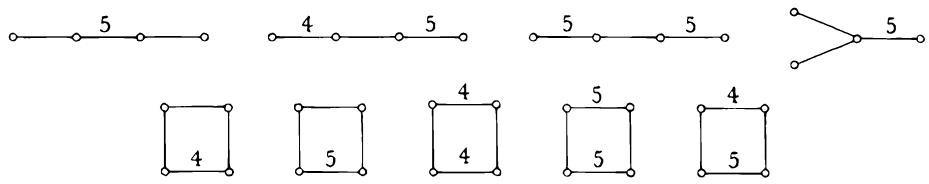
\includegraphics[keepaspectratio]{images/part001_8fab2eba.jpg}}

\begin{enumerate}
\def\labelenumi{\alph{enumi})}
\setcounter{enumi}{1}
\tightlist
\item
  The same question for rank 5, the list consisting of the following five graphs:
\end{enumerate}

\pandocbounded{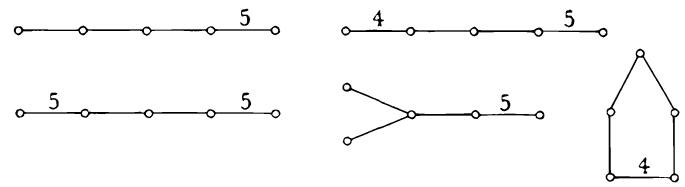
\includegraphics[keepaspectratio]{images/part001_6b3cac07.jpg}}

\begin{enumerate}
\def\labelenumi{\alph{enumi})}
\setcounter{enumi}{2}
\tightlist
\item
  Show that there is no graph of compact hyperbolic type of rank \(\geqslant 6\) .*
\end{enumerate}

\begin{enumerate}
\def\labelenumi{\arabic{enumi})}
\setcounter{enumi}{15}
\tightlist
\item
  *Show that any Coxeter graph of hyperbolic type of rank \(\geqslant 4\) that has an edge with coefficient 6 is isomorphic to one of the following eleven graphs (which are non-compact and of rank 4):
\end{enumerate}

\pandocbounded{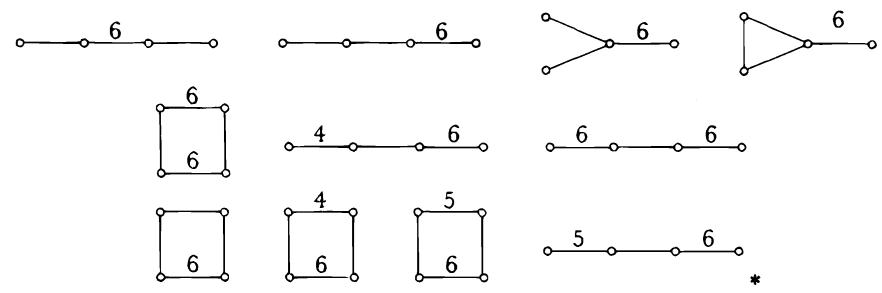
\includegraphics[keepaspectratio]{images/part001_2926a96c.jpg}}

\begin{enumerate}
\def\labelenumi{\arabic{enumi})}
\setcounter{enumi}{16}
\tightlist
\item
  *Show that the hyperbolic Coxeter graphs of higher rank are the following three graphs (which are of rank 10):
\end{enumerate}

\pandocbounded{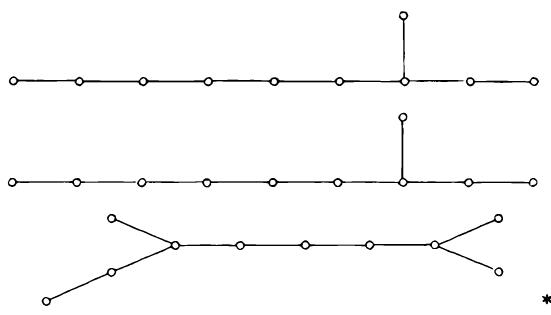
\includegraphics[keepaspectratio]{images/part001_3a8f46b0.jpg}}

¶ 18) Assume that (W,S) is of hyperbolic type, and that W leaves stable a lattice \(\Gamma\) of E. Let G be the orthogonal group of \(B_{M}\) , and let \(G(\Gamma)\) be the subgroup of elements \(g \in G\) such that \(g\Gamma = \Gamma\) . Show that \(G(\Gamma)\) is a discrete subgroup of G. Show that W is a subgroup of finite index of \(G(\Gamma)\) (use the fact that the measure of W\textbackslash G is finite).

*If (W, S) is actually of compact hyperbolic type, show that the corresponding Coxeter graph is isomorphic to one of the following (use Exercs. 4, 6 and 15):

\pandocbounded{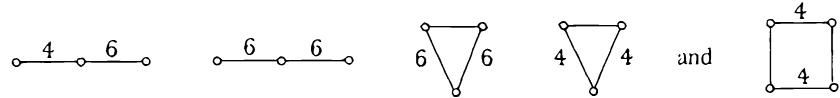
\includegraphics[keepaspectratio]{images/part001_0d92fd3d.jpg}}

Show that all the groups corresponding to the graphs of Exerc. 16 (with the exception of the last four) leave stable a lattice (use the method of Exerc. 6).*

\begin{enumerate}
\def\labelenumi{\arabic{enumi})}
\setcounter{enumi}{18}
\tightlist
\item
  Let \((W,S)\) be the Coxeter system corresponding to the graph
\end{enumerate}

\pandocbounded{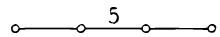
\includegraphics[keepaspectratio]{images/part001_8b3dcc37.jpg}}

This is a system of compact hyperbolic type (cf.~Exerc. 15). The coefficients of the form \(B_{M}\) with respect to the basis \((e_{s})\) belong to the subring A of the field \(\mathbf{Q}(\sqrt{5})\) consisting of the elements of this field that are integers over Z.

\begin{enumerate}
\def\labelenumi{\alph{enumi})}
\item
  Let \(\sigma\) be the embedding of \(K\) into \(\mathbf{R}\) that maps \(\sqrt{5}\) to \(-\sqrt{5}\) . Show that the transform \(\sigma(B_M)\) of the form \(B_M\) by \(\sigma\) is non-degenerate and positive.
\item
  Let G be the orthogonal group of \(B_{M}\) , and let \(G_{\sigma}\) be that of \(\sigma(B_{M})\) . Let \(G_{A}\) be the subgroup of G consisting of the elements whose matrices with respect to \((e_{s})\) have coefficients in A. Show that \(G_{A}\) can be identified with a discrete subgroup of \(G \times G_{\sigma}\) and then, using a), show that \(G_{A}\) is a discrete subgroup of G.
\item
  Show that W is a subgroup of \(G_{A}\) of finite index.
\end{enumerate}

\(d)\) Prove analogous results for the other graphs in Exerc. 15 (the field \(\mathbf{Q}(\sqrt{5})\) sometimes being replaced by \(\mathbf{Q}(\sqrt{2})\) , with the exception of the graph

\pandocbounded{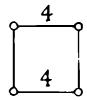
\includegraphics[keepaspectratio]{images/part001_99b486d1.jpg}}

treated in Exerc. 18, and of the graph \(^{8}\)

\pandocbounded{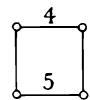
\includegraphics[keepaspectratio]{images/part001_2a5e784a.jpg}}

¶ 20) For every subset \(\{s, s'\}\) of S such that \(m(s, s') = \infty\) , let \(r(s, s')\) be a real number \(\leqslant -1\) . Equip E with the bilinear form \(\mathbf{B}_r\) such that

\[
\begin{array}{l l} \mathrm{B} _ {r} (e _ {s}, e _ {s ^ {\prime}}) = \mathrm{B} _ {\mathrm{M}} (e _ {s}, e _ {s ^ {\prime}}) = - \cos \frac {\pi}{m (s , s ^ {\prime})} & \text {if} m (s, s ^ {\prime}) \neq \infty \\ \mathrm{B} _ {r} (e _ {s}, e _ {s ^ {\prime}}) = r (s, s ^ {\prime}) & \text {if} m (s, s ^ {\prime}) = \infty . \end{array}
\]

We define, as for \(B_{M}\) , the reflections \(\sigma_{s}\) with vector \(e_{s}\) , leaving the form \(B_{r}\) invariant.

\begin{enumerate}
\def\labelenumi{\alph{enumi})}
\item
  Show that there exists a unique homomorphism \(\sigma_r: \mathbf{W} \to \mathbf{GL}(\mathbf{E})\) such that \(\sigma_r(g_s)\) is equal to the reflection \(\sigma_s\) defined above.
\item
  Show that the assertions in Prop. 4, Th. 1, its Corollaries, and Lemma 1 remain true for \(\sigma_r\) .
\end{enumerate}

\exercisesection{Exercises for § 5}

\begin{enumerate}
\def\labelenumi{\arabic{enumi})}
\item
  Determine the algebra of symmetric invariants of a finite dihedral group (for its canonical representation of dimension 2, cf.~§4, no. 2).
\item
  Let A be a principal ring, E a free A-module of finite rank l, and G a finite subgroup of \(\mathbf{GL}(\mathbf{E})\) . Assume the following:
\end{enumerate}

\begin{enumerate}
\def\labelenumi{(\roman{enumi})}
\item
  If \(q = \operatorname{Card}(G)\) , the element \(q.1\) of \(A\) is invertible.
\item
  G is generated by pseudo-reflections in E (i.e.~by elements s such that \((s - 1)(E)\) is a monogenic submodule of E, cf.~§2, Exerc. 1.)
\end{enumerate}

Let \(\mathbf{S}(\mathrm{E})\) be the symmetric algebra of \(\mathrm{E}\) , and let \(\mathbf{S}(\mathrm{E})^{\mathrm{G}}\) be the subalgebra of \(\mathbf{S}(\mathrm{E})\) consisting of the elements invariant under \(\mathrm{G}\) . Show that, for any homomorphism from \(\mathrm{A}\) into a field \(k\) , \(\mathbf{S}(\mathrm{E})^{\mathrm{G}} \otimes k\) can be identified with \(\mathbf{S}(\mathrm{E} \otimes k)^{\mathrm{G}}\) . Deduce, by applying Th. 4, that \(\mathbf{S}(\mathrm{E})^{\mathrm{G}}\) is a graded polynomial algebra over \(\mathrm{A}\) .

¶ 3) Let K be a field of characteristic zero, V a vector space of finite dimension l over K, and G a subgroup of GL(V) generated by pseudo-reflections. Put q = Card(G); denote by S (resp. L) the symmetric algebra (resp. exterior algebra) of V. If \(x \in V\) , denote by x (resp. \(x'\) ) its canonical image in S (resp. L).

\begin{enumerate}
\def\labelenumi{\alph{enumi})}
\item
  Let \(E = S \otimes L\) be the tensor product of S and L. Show that there exists a unique derivation d on E such that \(dx = x'\) and \(dx' = 0\) for all \(x \in V\) .
\item
  Let \(S^{G}\) be the algebra of symmetric invariants of G and let \(P_{1},\ldots,P_{l}\) be homogeneous elements of \(S^{G}\) such that \(S^{G}=K[P_{1},\ldots,P_{l}]\) . For every subset \(I=\{i_{1},\ldots,i_{r}\}\) of \([1,l]\) with \(i_{1}<\cdots<i_{r}\) , put
\end{enumerate}

\[
\omega_ {\mathrm{I}} = d \mathrm{P} _ {i _ {1}} \dots d \mathrm{P} _ {i _ {r}}.
\]

Show that the \(\omega_{I}\) are linearly independent over S, and that they belong to the subalgebra \(E^{G}\) consisting of the elements of E invariant under G. Deduce that, for all \(\omega \in E^{G}\) , there exist \(a, c_{I} \in S^{G}\) , with \(a \neq 0\) , such that

\[
a \omega = \sum_ {\mathrm{I}} c _ {\mathrm{I}} \omega_ {\mathrm{I}}.
\]

\(c)\) Show that every element of \(\mathrm{E}^{\mathrm{G}}\) contained in \(S\otimes \bigwedge^{l}\mathrm{V}\) is of the form \(c.dP_{1}\ldots dP_{l}\) , with \(c\in S^{\mathrm{G}}\) . (Apply Prop. 5.)

\begin{enumerate}
\def\labelenumi{\alph{enumi})}
\setcounter{enumi}{3}
\item
  Show that the \(\omega_{I}\) form a basis of the \(S^{G}\) -module \(E^{G}\) . (With the notation in b), multiply both sides of the relation \(a\omega = \sum_{I} c_{I}\omega_{I}\) by an element \(\omega_{J}\) , and apply c); deduce that, if I is the complement of J, a divides \(c_{I}\) ; hence \(^{9}\) the fact that the \(\omega_{I}\) generate \(E^{G}\) .)
\item
  Let \(S_{n}\) (resp. \(L_{m}\) ) be the homogeneous component of \(S\) (resp. \(L\) ) of degree \(n\) (resp. \(m\) ). Put
\end{enumerate}

\[
\begin{array}{r l r} & & {\mathrm{E} _ {n, m} = \mathrm{S} _ {n} \otimes \mathrm{L} _ {m}, \quad \mathrm{E} _ {n, m} ^ {\mathrm{G}} = \mathrm{E} ^ {\mathrm{G}} \cap \mathrm{E} _ {n, m}, \quad a _ {n, m} = \dim \mathrm{E} _ {n, m} ^ {\mathrm{G}},} \\ & & {a (\mathrm{X}, \mathrm{Y}) = \sum_ {n, m \geqslant 0} a _ {n, m} \mathrm{X} ^ {n} \mathrm{Y} ^ {m}.} \end{array}
\]

By using \(d\) ), prove the formula

\[
a (\mathrm{X}, \mathrm{Y}) = \prod_ {i = 1} ^ {l} \frac {1 + \mathrm{Y} . \mathrm{X} ^ {p _ {i} - 1}}{1 - \mathrm{X} ^ {p _ {i}}},
\]

where \(p_{i} = \deg(P_{i})\) .

\(f)\) If \(g \in \mathbf{G}\) , let \(\operatorname{Tr}_{n,m}(g)\) be the trace of the automorphism of \(\mathbf{E}_{n,m}\) defined by \(g\) ; put

\[
\operatorname{Tr} (\mathrm{X}, \mathrm{Y}) (g) = \sum_ {n, m \geqslant 0} \operatorname{Tr} _ {n, m} (g) \mathrm{X} ^ {n} \mathrm{Y} ^ {m}.
\]

Show that

\[
\operatorname{Tr} (X, Y) (g) = \frac {\det (1 + Y g)}{\det (1 - X g)}.
\]

\begin{enumerate}
\def\labelenumi{\alph{enumi})}
\setcounter{enumi}{6}
\tightlist
\item
  Let \(q = \operatorname{Card}(\mathbf{G})\) . Show that
\end{enumerate}

\[
\frac {1}{q} \sum_ {g \in G} \operatorname{Tr} (X, Y) (g) = a (X, Y),
\]

i.e.

\[
\frac {1}{q} \sum_ {g \in G} \frac {\det (1 + Y g)}{\det (1 - X g)} = \prod_ {i = 1} ^ {l} \frac {1 + Y . X ^ {p _ {i} - 1}}{1 - X ^ {p _ {i}}}.
\]

(Use the following result: if \(\mathbf{G}\) acts on a finite dimensional vector space \(\mathbf{E}\) , the dimension of the space of elements of \(\mathbf{E}\) invariant under \(\mathbf{G}\) is equal to \(\frac{1}{q}\sum_{g\in \mathbf{G}}\mathrm{Tr}_{\mathbf{E}}(g).\) )

What does this formula give for Y = 0?

\begin{enumerate}
\def\labelenumi{\alph{enumi})}
\setcounter{enumi}{7}
\tightlist
\item
  For any integer \(p \geqslant 0\) , let \(H_{p}\) be the set of elements \(g \in G\) that have 1 as an eigenvalue with multiplicity p.~Let \(h_{p} = \text{Card}(H_{p})\) . Prove the formula
\end{enumerate}

\[
\sum_ {p = 0} ^ {l} h _ {p} \mathbf {T} ^ {p} = \prod_ {i = 1} ^ {l} (p _ {i} - 1 + \mathbf {T}).
\]

(In the formula in \(g\) ) above, replace \(Y\) by \(-1 + T(1 - X)\) and then put \(X = 1\) in the result. If \(g \in H_p\) , the term \(\operatorname{Tr}(X, Y)(g)\) becomes \(T^p\) .)

¶ 4) *Let \(G _ {1} = \mathbf {S L} _ {3} (\mathbf {F} _ {2})\).

\begin{enumerate}
\def\labelenumi{\alph{enumi})}
\item
  Show that \(\mathbf{G}_1\) is a non-abelian simple group of order 168, containing 21 elements of order 2.
\item
  Show that the degrees of the irreducible complex representations of \(G_{1}\) are 1, 3, 3, 6, 7, 8.
\item
  Let \(\rho: \mathbf{G}_1 \to \mathbf{GL}_3(\mathbf{C})\) be an irreducible representation \(^{10}\) of \(\mathbf{G}_1\) of degree 3. If \(y \in \mathbf{G}_1\) is of order 2, show that \(\operatorname{Tr}(\rho(y)) = -1\) . Deduce that \(-\rho(y)\) is a reflection.
\item
  Let G be the subgroup of \(\mathbf{GL}_{3}(\mathbf{C})\) generated by the elements \(-\rho(y)\) , for y of order 2 in \(G_{1}\) . Show that G is isomorphic to \(G_{1} \times \{1, -1\}\) , and is thus of order 336.
\item
  Show that the characteristic degrees \(k_{1}, k_{2}, k_{3}\) of the algebra of symmetric invariants of \(\mathbf{G}\) are equal to 4, 6 and 14. (Use the relations \(\prod_{i} k_{i} = 336\) and \(\sum_{i} (k_{i} - 1) = 21\) .)
\item
  Show that G is not a Coxeter group.*
\end{enumerate}

\begin{enumerate}
\def\labelenumi{\arabic{enumi})}
\setcounter{enumi}{4}
\tightlist
\item
  *Let \(K\) be a field and \(S = K[X_1, \ldots, X_n]\) a graded polynomial algebra over \(K\) , generated by algebraically independent elements \(X_i\) , homogeneous of degrees \(> 0\) .
\end{enumerate}

\begin{enumerate}
\def\labelenumi{\alph{enumi})}
\tightlist
\item
  Let \(Y_{1},\ldots,Y_{n}\) be homogeneous elements of S of degrees \textgreater0, and let \(R = K[Y_{1},\ldots,Y_{n}]\) be the subalgebra of S generated by these elements. Prove the equivalence of the following properties:
\end{enumerate}

\begin{enumerate}
\def\labelenumi{(\roman{enumi})}
\item
  \((\mathrm{Y}_1,\dots ,\mathrm{Y}_n)\) is an S-regular sequence.
\item
  S is integral over R.
\item
  The ideal of \(S\) generated by \(Y_{1},\ldots ,Y_{n}\) is of finite codimension in \(S\) .
\item
  For any extension \(\overline{\mathbf{K}}\) of \(\mathbf{K}\) , the system of equations \(Y_{i}(x_{1},\ldots ,x_{n}) = 0\) ( \(1\leqslant i\leqslant n\) , \(x_{i}\in \overline{\mathbf{K}}\) ) has only the trivial solution \((0,\dots ,0)\) .
\end{enumerate}

\(((\mathrm{i}) \Longleftrightarrow (\mathrm{iii})\) follows from a theorem of Macaulay (Commutative Algebra); \((\mathrm{iii}) \Longleftrightarrow (\mathrm{iv})\) follows from the Zeros Theorem (Commutative Algebra, Chap. V, §3, no. 3, Prop. 2); (ii) \(\Longleftrightarrow (\mathrm{iii})\) is easy.)

If these properties are satisfied, show that the \(Y_{i}\) are algebraically independent over K, and that S is a free R-module of rank equal to

\[
\frac {\prod_ {i} \deg (\mathrm{Y} _ {i})}{\prod_ {i} \deg (\mathrm{X} _ {i})}.
\]

\begin{enumerate}
\def\labelenumi{\alph{enumi})}
\setcounter{enumi}{1}
\tightlist
\item
  Let G be a finite group of automorphisms of the graded algebra S, let \(S^{G}\) be its subalgebra of invariants, and let \(Y_{1},\ldots,Y_{n}\) be elements of \(S^{G}\) satisfying conditions (i),\ldots, (iv) above. Show that \(S^{G}=K[Y_{1},\ldots,Y_{n}]\) if and only if
\end{enumerate}

\[
\operatorname{Card} (\mathrm{G}) = \frac {\prod_ {i} \deg \left(\mathrm{Y} _ {i}\right)}{\prod_ {i} \deg \left(\mathrm{X} _ {i}\right)}. *
\]

¶ 6) *Let n be an integer ≥ 1, q a power of a prime number, K = F\_q, V = K\^{}n, G = GL(n, K) and G\_1 = SL(n, K). Identify G with the group GL(V). Further, denote by S the algebra S(V) = K{[}X\_1, \ldots, X\_n{]} and R (resp. R\_1) the subalgebra of S consisting of the elements invariant under G (resp. G\_1).

\begin{enumerate}
\def\labelenumi{\alph{enumi})}
\tightlist
\item
  Let \(\mathbf{e} = (e_1, \ldots, e_n)\) be a sequence of integers \(\geqslant 0\) . Put
\end{enumerate}

\[
\mathrm{L} _ {\mathbf {e}} = \det (\mathrm{X} _ {i} ^ {q ^ {e _ {j}}}).
\]

This is an element of \(S\) .

Show that

\[
g. \mathrm{L} _ {\mathbf {e}} = \det (g) \mathrm{L} _ {\mathbf {e}} \text {for all} g \in \mathrm{G}.
\]

(Remark that, if \(g.X_i = \sum_j a_{ij} X_j\) , then \(g.X_i^{q^e} = \sum_j a_{ij} X_j^{q^e}\) .) In particular, \(L_e\) belongs to \(R_1\) .

\begin{enumerate}
\def\labelenumi{\alph{enumi})}
\setcounter{enumi}{1}
\tightlist
\item
  Let \(j \in [1, n]\) . Put
\end{enumerate}

\[
Z _ {j} = \prod_ {(a _ {i j})} (X _ {j} + \sum_ {i > j} a _ {i j} X _ {i}),
\]

the product being over all families \((a_{ij})_{j < i\leqslant n}\) of elements of K. Let

\[
\mathrm{T} = \prod_ {j = 1} ^ {n} Z _ {j}.
\]

Show that T divides all the \(L_{e}\) . Deduce that \(T = L_{e_{n}}\) , where \(e_{n} = (0, 1, \ldots, n - 1)\) , and that T is invariant under \(G_{1}\) .

\begin{enumerate}
\def\labelenumi{\alph{enumi})}
\setcounter{enumi}{2}
\tightlist
\item
  Denote by \(\mathbf{e}_i\) ( \(1 \leqslant i \leqslant n - 1\) ) the sequence \((0, 1, \ldots, i - 1, i + 1, \ldots, n)\) , and put \(\mathrm{Y}_i = \mathrm{L}_{\mathbf{e}_i} / \mathrm{T}\) , cf.~b). Show that the \(\mathrm{Y}_i\) belong to R and that \(\deg(\mathrm{Y}_i) = q^n - q^i\) .
\end{enumerate}

\(d)\) Let \(S' = K[X_1, \ldots, X_{n-1}]\) , and let \(T', Y_1', \ldots, Y_{n-2}'\) be the elements of \(S'\) defined in the same way as \(T, Y_1, \ldots, Y_{n-1}\) (but replacing \(n\) by \(n-1\) ). Let \(f: S \to S'\) be the homomorphism defined by

\[
f \left(\mathrm{X} _ {i}\right) = \mathrm{X} _ {i} (1 \leqslant i \leqslant n - 1), f \left(\mathrm{X} _ {n}\right) = 0.
\]

Show that

\[
f (\mathrm{T}) = 0, \quad f (\mathrm{Y} _ {1}) = \mathrm{T} ^ {\prime q (q - 1)}, \quad f (\mathrm{Y} _ {i}) = \mathrm{Y} _ {i - 1} ^ {\prime q} \quad \text{for} \quad 2 \leqslant i \leqslant n - 1.
\]

\begin{enumerate}
\def\labelenumi{\alph{enumi})}
\setcounter{enumi}{4}
\tightlist
\item
  Show that the family \((T, Y_{1}, \ldots, Y_{n-1})\) satisfies condition (iv) of Exerc. 5. (Let \(x = (x_{1}, \ldots, x_{n})\) be a zero of the system \((T, Y_{1}, \ldots, Y_{n-1})\) in an extension \(\overline{K}\) of K. Since x is a zero of T, the \(x_{i}\) satisfy at least one non-trivial linear relation with coefficients in K. Transforming x by an element of \(G_{1}\) if necessary, we can assume that \(x_{n} = 0\) . Conclude by applying d) and arguing by induction on n.)
\end{enumerate}

\(f)\) Show that \(\mathbf{R}_1 = \mathbf{K}[\mathbf{T},\mathbf{Y}_1,\dots ,\mathbf{Y}_{n - 1}]\) , and that \(\mathrm{T},\mathrm{Y}_1,\dots ,\mathrm{Y}_{n - 1}\) are algebraically independent (``Dickson's Theorem'' - apply e) and Exerc. 5, remarking that the order of \(\mathbf{G}_1\) is equal to \(\deg (\mathrm{T}) = \sum_{i}\deg (\mathrm{Y}_i)\)).

\begin{enumerate}
\def\labelenumi{\alph{enumi})}
\setcounter{enumi}{6}
\tightlist
\item
  Show that \(R = K[T^{q-1}, Y_{1}, \ldots, Y_{n-1}]\) .
\end{enumerate}

¶ 7) *Let R be a regular local ring (Commutative Algebra, Chap. VIII, §5, no. 1), with maximal ideal m and residue field k. Let G be a finite group of automorphisms of R, and let \(R' = R^{G}\) be the subring of R consisting of the elements invariant under G. This is a local ring with maximal ideal \(m' = m \cap R'\) . Assume the following:

\begin{enumerate}
\def\labelenumi{(\roman{enumi})}
\item
  \(R'\) is noetherian and R is an \(R'\) -module of finite type.
\item
  The composite \(R'\to R\to k\) is surjective.
\end{enumerate}

Put \(V = \mathfrak{m} / \mathfrak{m}^2\) ; this is a \(k\) -vector space. The action of \(G\) on \(R\) defines a homomorphism \(\varepsilon : G \to \mathbf{GL}(V)\) .

\begin{enumerate}
\def\labelenumi{\alph{enumi})}
\item
  Let \(\mathfrak{p}\) be a prime ideal of \(R\) of height 1 (Commutative Algebra, Chap. VII, §1, no. 6) and let \(s \in G\) be such that \(s(\mathfrak{p}) = \mathfrak{p}\) and that \(s\) acts trivially on \(R / \mathfrak{p}\) . Show that \(\varepsilon(s)\) is a pseudo-reflection of \(V\) . (Remark that the image of \(\mathfrak{p}\) in \(\mathfrak{m} / \mathfrak{m}^2\) is of dimension 0 or 1.)
\item
  Show that, if \(R'\) is regular, the subgroup \(\varepsilon(G)\) of \(\mathbf{GL}(V)\) is generated by pseudo-reflections, (Let H be the subgroup of G generated by elements whose image under \(\varepsilon\) is a pseudo-reflection, and let \(R^{H}\) be the subring of R consisting of elements invariant under H. Show, using a), that no prime ideal of \(R'\) of height 1 is ramified in \(R^{H}\) ; using the fact that \(R^{H}\) is integrally closed, deduce by means of the Purity Theorem \(^{11}\) that \(R' = R^{H}\) , so H = G.)
\item
  Assume now that the order of \(\mathbf{G}\) is coprime to the characteristic of \(k\) . Show that \(\varepsilon\) is injective.
\end{enumerate}

Let \((\mathfrak{m}_{n}^{\prime})\) be the filtration of \(R^{\prime}\) induced by the m-adic filtration \((\mathfrak{m}^{n})\) of R, and let

\[
i: \mathrm{gr} (\mathrm{R} ^ {\prime}) \to \mathrm{gr} (\mathrm{R})
\]

be the canonical homomorphism of the associated graded algebra of \(R'\) to that of R (Commutative Algebra, Chap. III, §2). Show that i is injective, and that its image is the subring \(\mathrm{gr}(R)^{\mathrm{G}}\) of \(\mathrm{gr}(R)\) consisting of the elements invariant under G.

\(d)\) Retain the assumptions and notation of \(c\) ), and assume further that \(\varepsilon (\mathbf{G})\) is generated by pseudo-reflections. If \(l = \dim V\) , let \(\mathrm{P}_1,\ldots ,\mathrm{P}_l\) be algebraically independent homogeneous generators of the \(k\) -algebra \(\mathrm{gr}(R)^{\mathrm{G}}\) (such elements exist by Th. 4 and the fact that \(\mathrm{gr}(R)\) can be identified with the symmetric algebra of V); let \(p_1,\ldots ,p_l\) be their degrees. By \(c\) ), we can find \(x_{i}\in \mathfrak{m}_{p_{i}}^{\prime}\) such that \(\mathrm{gr}(x_i) = \mathrm{P}_i\) . Show that the \(x_{i}\) generate the ideal \(\mathfrak{m}'\) and deduce that \(R'\) is regular.*

¶ 8) *Let V be a finite dimensional vector space over a field K, let S be the symmetric algebra of V, and let G be a finite subgroup of GL(V). Assume that the algebra \(S^G\) of symmetric invariants of \(G\) is a graded polynomial algebra.

\begin{enumerate}
\def\labelenumi{\alph{enumi})}
\tightlist
\item
  Let u be an element of the dual \(V^{*}\) of V, and let \(G_{u}\) be the subgroup of G consisting of the elements leaving u invariant. Show that \(G_{u}\) is generated by pseudo-reflections. (The linear form u extends to a homomorphism \(f_{u}: S \to K\) . If \(S_{u}\) denotes the local ring of S with respect to the kernel of \(f_{u}\) , the ring \(S_{u}\) is regular. Conclude by applying Exerc. 7 b) to \(G_{u}\) , considered as a group of automorphisms of \(S_{u}\) .)
\end{enumerate}

In particular, G is generated by pseudo-reflections.

\begin{enumerate}
\def\labelenumi{\alph{enumi})}
\setcounter{enumi}{1}
\tightlist
\item
  Let A be a subset of \(V^{*}\) , and let \(G_{A} = \bigcap_{u \in A} G_{u}\) . Show that \(G_{A}\) is generated by pseudo-reflections. (Extending the base field if necessary, we can assume that K is infinite. Show that in that case there exists an element v of the vector subspace of \(V^{*}\) generated by A such that \(G_{v} = G_{A}\) . Conclude by applying a) to \(v\) .)
\end{enumerate}

\begin{enumerate}
\def\labelenumi{\arabic{enumi})}
\setcounter{enumi}{8}
\tightlist
\item
  Let V be a vector space of dimension 4 over a finite field K, of characteristic different from 2, and let Q be a non-degenerate quadratic form on V of index 2 (Algebra, Chap. IX, §4, no. 2). Let G = O(Q) be the orthogonal group of this form; this is a finite group generated by reflections (loc. cit., §6, no. 4, Prop. 5).
\end{enumerate}

\begin{enumerate}
\def\labelenumi{\alph{enumi})}
\item
  Let E be a maximal totally isotropic subspace of V, and let \(G_{E}\) be the subgroup of G consisting of the elements g such that \(g(x) = x\) for all \(x \in E\) . Show that \(G_{E}\) is isomorphic to the additive group of K, and contains no pseudo-reflection.
\item
  Show that the algebra of symmetric invariants of G is not a graded polynomial algebra (use the preceding exercise).
\end{enumerate}

\exercisesection{Exercises for § 6}

In the exercises below (with the exception of Exerc. 3), the assumptions and notation are those of §6.

\begin{enumerate}
\def\labelenumi{\arabic{enumi})}
\item
  Assume that W is irreducible. Let c be a Coxeter transformation of W, let \(\Gamma\) be the subgroup of W generated by c, and let \(\Delta\) be the set of unit vectors orthogonal to an element of H. Show that \(\Gamma\) has l orbits in \(\Delta\) , and that each orbit has h elements. (Argue as in the proof of Prop. 33 of Chap. VI, §1, no. 11.)
\item
  Assume that W is irreducible. Let C be a chamber relative to W, \((\mathrm{H}_{1},\ldots,\mathrm{H}_{l})\) its walls, and \(e_{i}\) a non-zero vector orthogonal to \(H_{i}\) . Assume that \(e_{1},\ldots,e_{r}\) (resp. \(e_{r+1},\ldots,e_{l}\) ) are pairwise orthogonal (cf.~no. 2). For all \(u\in Z\) , define \(H_{u}\) and \(s_{u}\) by \(H_{u}=H_{k}\) if \(u\equiv k\pmod{l}\) and \(s_{u}=s_{H_{u}}\) .
\end{enumerate}

\begin{enumerate}
\def\labelenumi{\alph{enumi})}
\item
  Show that the elements of \(\mathfrak{H}\) are the \(s_1 s_2 \ldots s_{u-1} H_u\) for \(u = 1, 2, \ldots, lh/2\) .
\item
  Let \(s' = s_1 \ldots s_r\) and \(s'' = s_{r+1} \ldots s_l\) , so that \(c = s's''\) is the Coxeter transformation associated to the ordered chamber C. Let \(w_0\) be the element of W that transforms C to -C (cf.~§4, Exerc. 2). Show that, if \(h\) is odd,
\end{enumerate}

\[
w _ {0} = \underbrace {s ^ {\prime} s ^ {\prime \prime} s ^ {\prime} \ldots s ^ {\prime \prime} s ^ {\prime}} _ {h \text {terms}} = \underbrace {s ^ {\prime \prime} s ^ {\prime} s ^ {\prime \prime} \ldots s ^ {\prime} s ^ {\prime \prime}} _ {h \text {terms}} = s ^ {\prime \prime} c ^ {(h - 1) / 2} = c ^ {(h - 1) / 2} s ^ {\prime}.
\]

\begin{enumerate}
\def\labelenumi{\alph{enumi})}
\setcounter{enumi}{2}
\tightlist
\item
  Put \(S = \{s_1, \ldots, s_l\}\) . The pair (W,S) is a Coxeter system. If \(w \in W\) , denote by \(l_S(w)\) the length of \(w\) with respect to S (Chap. IV, §1, no. 1). Show that
\end{enumerate}

\[
l _ {\mathrm{S}} (s ^ {\prime}) = r, l _ {\mathrm{S}} (s ^ {\prime \prime}) = l - r, l _ {\mathrm{S}} (c) = l.
\]

Deduce that, with the assumptions in b).

\[
l _ {\mathrm{S}} (w _ {0}) \leqslant r + \frac {h - 1}{2} l \text { and } l _ {\mathrm{S}} (w _ {0}) \leqslant (l - r) + \frac {h - 1}{2} l.
\]

Show on the other hand that \(l_{S}(w_0) = \mathrm{Card}(\mathfrak{H}) = hl / 2\) (use Exerc. 22 of Chap. IV, §1). Deduce that \(r = l / 2\) and that \((s_1, s_2, \ldots, s_{lh / 2})\) is a reduced decomposition of \(w_0\) .

\(d)\) Show that, if \(h\) is even, \((s_1,\ldots ,s_{lh / 2})\) is a reduced decomposition of \(w_{0} = c^{h / 2}\) . (Same method.)

¶ 3) Let K be a commutative ring, E a free K-module with basis \((e_1, \ldots, e_l)\) , and \(f_1, \ldots, f_l\) elements of the dual of E. Put \(a_{ij} = f_i(e_j)\) . If \(1 \leqslant i \leqslant l\) , let \(s_i\) be the pseudo-reflection \(s_{e_i, f_i}\) (\S 2, Exerc. 1). Then

\[
s _ {i} (e _ {j}) = e _ {j} - a _ {i j} e _ {i}.
\]

Put \(c = s_1 \ldots s_l\) , and \(z_i = c(e_i)\) .

\begin{enumerate}
\def\labelenumi{\alph{enumi})}
\tightlist
\item
  For \(1 \leqslant i, k \leqslant l\) , put
\end{enumerate}

\[
y _ {i} ^ {k} = s _ {1} \dots s _ {k} (e _ {i}) \text { and } y _ {i} = s _ {1} \dots s _ {i - 1} (e _ {i}) = y _ {i} ^ {i - 1}.
\]

Thus \(y_{i}^{0} = e_{i}\) and \(y_{i}^{l} = z_{i}\) .

Show that

\[
y _ {i} ^ {k - 1} - y _ {i} ^ {k} = a _ {k i} y _ {k}.
\]

Deduce the formulas

\[
e _ {i} = y _ {i} + \sum_ {k <   i} a _ {k i} y _ {k}
\]

\[
z _ {i} = y _ {i} - \sum_ {k \geqslant i} a _ {k i} y _ {k}.
\]

\begin{enumerate}
\def\labelenumi{\alph{enumi})}
\setcounter{enumi}{1}
\tightlist
\item
  Let C be the matrix of \(c\) with respect to the basis \((e_i)\) . Let \(U = (u_{ij})\) and \(V = (v_{ij})\) be the matrices defined by
\end{enumerate}

\[
u _ {i j} = \left\{ \begin{array}{l l} a _ {i j} & \text { if } i <   j \\ 0 & \text { otherwise, } \end{array} \right. v _ {i j} = \left\{ \begin{array}{l l} 0 & \text { if } i <   j \\ a _ {i j} & \text { otherwise. } \end{array} \right.
\]

The matrix \(\mathrm{I} + \mathrm{U}\) is invertible with determinant 1. Show that

\[
\mathrm{C} = (\mathrm{I} - \mathrm{V}) (\mathrm{I} + \mathrm{U}) ^ {- 1}.
\]

Deduce that

\[
\det (\lambda I - C) = \det ((\lambda - 1) I + V + \lambda U),
\]

in other words

\[
\det (\lambda \mathrm{I} - \mathrm{C}) = \left| \begin{array}{c c c c c} (\lambda - 1) + a _ {1 1} & \lambda a _ {1 2} & \lambda a _ {1 3} & \dots & \lambda a _ {1 l} \\ a _ {2 1} & \lambda (\lambda - 1) + a _ {2 2} & \lambda a _ {2 3} & \dots & \lambda a _ {2 l} \\ a _ {3 1} & a _ {3 2} & (\lambda - 1) + a _ {3 3} & \dots & \lambda a _ {3 l} \\ \vdots & \vdots & \vdots & \ddots & \vdots \\ a _ {l 1} & a _ {l 2} & a _ {l 3} & \dots & (\lambda - 1) + a _ {l l} \end{array} \right|.
\]

\begin{enumerate}
\def\labelenumi{\alph{enumi})}
\setcounter{enumi}{2}
\tightlist
\item
  Let \(\Gamma = (\mathrm{I},\mathrm{S})\) be the graph whose set of vertices is \(\mathrm{I} = [1,l]\) and whose set S of arrows is the set of subsets \(\{i,j\}\) of I with 2 elements such that \(a_{ij}\neq 0\) or \(a_{ji}\neq 0\) . If \(\alpha = \{i,j\}\) belongs to S, denote by \(\sigma_{\alpha}\) the transposition of \(i\) and \(j\) (considered as an element of the symmetric group \(\mathrm{S_I}\) ), and put \(a_{\alpha} = -a_{ij}a_{ji}\) .
\end{enumerate}

Let \(\mathfrak{B}\) be the set of subsets of \(S\) consisting of the arrows whose vertices are disjoint. If \(X \in \mathfrak{B}\) , denote by \(C(X)\) the set of \(i \in I\) that are not vertices of any arrow of \(X\) , and put \(\sigma_X = \prod_{\alpha \in X} \sigma_\alpha\) , \(a_X = \prod_{\alpha \in X} a_\alpha\) .

Let \(\sigma \in S_{I}\) , and let \(d_{\sigma}\) be the term corresponding to \(\sigma\) in the expansion of the determinant of \((\lambda - 1)I + V + \lambda U\) . Show that, if \(\sigma\) is of the form \(\sigma_{X}\) , with \(X \in \mathfrak{B}\) , then

\[
d _ {\sigma} = a _ {X} \lambda^ {\operatorname{Card} (X)} \prod_ {i \in C (X)} (\lambda - 1 + a _ {i i}).
\]

Assume now that \(\Gamma\) is a forest (Chap. IV, Appendix, no. 3). Show that, if \(\sigma \in S_l\) is not of the form \(\sigma_X\) with \(X \in \mathfrak{B}\) , then \(d_{\sigma} = 0\) . Deduce the formula

\[
\det (\lambda - c) = \sum_ {X \in \mathfrak {B}} a _ {X} \lambda^ {\operatorname{Card} (X)} \prod_ {i \in C (X)} (\lambda - 1 + a _ {i i}).
\]

\begin{enumerate}
\def\labelenumi{\alph{enumi})}
\setcounter{enumi}{3}
\tightlist
\item
  Consider the polynomial
\end{enumerate}

\[
P (X) = \left| \begin{array}{c c c c} X & a _ {1 2} & \ldots & a _ {1 l} \\ a _ {2 1} & X & \ldots & a _ {2 l} \\ \vdots & \vdots & \ddots & \vdots \\ a _ {l 1} & a _ {l 2} & \ldots & X \end{array} \right|.
\]

To the assumptions in \(c\) ), we add that \(a_{ii} = 1\) for all \(i\) . Show that in that case

\[
\det (\lambda^ {2} - c) = \lambda^ {l} P (\lambda + \lambda^ {- 1}).
\]

\begin{enumerate}
\def\labelenumi{\arabic{enumi})}
\setcounter{enumi}{3}
\tightlist
\item
  With the assumptions and notation of no. 1, denote by \(n_{ij}\) the order of \(s_{\mathrm{H}_i}s_{\mathrm{H}_j}\) , and put \(a_{ij} = -2\cos \frac{\pi}{n_{ij}}\) . Then \(a_{ii} = 2\) and \(a_{ij} \leqslant 0\) if \(i \neq j\) , cf.~§3. Show \(^{12}\) , by using the method of the preceding exercise, that
\end{enumerate}

\[
\left| \begin{array}{c c c c} X & a _ {1 2} & \ldots & a _ {1 l} \\ a _ {2 1} & X & \ldots & a _ {2 l} \\ \vdots & \vdots & \ddots & \vdots \\ a _ {l 1} & a _ {l 2} & \ldots & X \end{array} \right| = \prod_ {i = 1} ^ {l} (X - 2 \cos (\pi m _ {i} / h)),
\]

where \(m_{1},\ldots ,m_{l}\) are the exponents of W.

\chapter{ROOT SYSTEMS}

\section{ROOT SYSTEMS}

In this paragraph, k denotes a field of characteristic zero. From no. 3 onwards, we assume that k = R.
